\documentclass[11pt]{amsart} %leqno
\usepackage[left=1.3in,right=1.3in,bottom=1.6in]{geometry}
%\linespread{1.1}
%\usepackage[explicit]{titlesec}
\usepackage{lipsum}
\usepackage{mathrsfs}

\usepackage{hyphenat}
\usepackage{graphicx}
\usepackage{tikz}
\usepackage{pgfplots}
\usetikzlibrary{shapes.geometric,fit,matrix}


\usepackage{array, booktabs, caption}
\usepackage{ragged2e}
\usepackage{multirow}
\usepackage{hhline}% http://ctan.org/pkg/hhline
\usepackage{makecell}
\usepackage{enumitem}
\usepackage{bbm}
\usepackage{soul}
\usepackage{mathtools}
\usepackage{commath}
\allowdisplaybreaks

\usepackage[citecolor=red]{hyperref}

\usepackage[normalem]{ulem}
\usepackage{relsize}




%\usepackage[nottoc]{tocbibind}
\usepackage[bottom]{footmisc}
%\usepackage{natbib}


\usepackage[normalem]{ulem}
\usepackage{relsize}
\usepackage{commath}
\usepackage{mathtools}
\allowdisplaybreaks

\title{Introduction to Algebra: Fall 2017}
\author{Meng Hsuan Hsieh}
\thanks{Based on undergraduate Algebra course taught by Robert Ji Wai Young. Please contact \url{menghsuan.hsieh@nyu.edu} for any typos, maths errors, and the like.}
\date{\today}

%\renewcommand\sectionmark[1]{\markleft{\thesection. #1}} % neither \markboth nor \markright work 



\usepackage{float}

\usepackage{color}

\usepackage{amsthm}

\newcommand\independent{\protect\mathpalette{\protect\independenT}{\perp}}
\def\independenT#1#2{\mathrel{\rlap{$#1#2$}\mkern2mu{#1#2}}}

\usepackage[utf8]{inputenc}
\usepackage[english]{babel}
\usepackage{textcomp}

\renewcommand\theadalign{lc}
\renewcommand\theadfont{\bfseries}
\usepackage{amssymb} %maths
\usepackage{amsmath} %maths
\usepackage{amsfonts}

\usepackage[utf8]{inputenc} %useful to type directly diacritic characters

\makeatletter
\renewcommand*\env@matrix[1][*\c@MaxMatrixCols c]{%
	\hskip -\arraycolsep
	\let\@ifnextchar\new@ifnextchar
	\array{#1}}
\makeatother

\theoremstyle{definition}
\newtheorem{definition}{Definition}[section]
\newtheorem{proposition}[definition]{Proposition}
\newtheorem{theorem}[definition]{Theorem}
\newtheorem{corollary}[definition]{Corollary}
\newtheorem{lemma}[definition]{Lemma}
\newtheorem{obs}[definition]{Observation}
\newtheorem{example}[definition]{Example}
\newtheorem{assumption}[definition]{Assumption}
\newtheorem{properties}[definition]{Properties}
\newtheorem{motivation}[definition]{Motivation}
\newtheorem{idea}[definition]{Idea}
\newtheorem{fact}[definition]{Fact}
\newtheorem{consequence}[definition]{Consequence}

\theoremstyle{definition}
\newtheorem{remark}[definition]{Remark}

\DeclareMathOperator{\N}{\mathbb{N}}
\DeclareMathOperator{\Q}{\mathbb{Q}}
\DeclareMathOperator{\R}{\mathbb{R}}
\DeclareMathOperator{\Z}{\mathbb{Z}}
\DeclareMathOperator{\F}{\mathbb{F}}
\DeclareMathOperator{\FF}{\mathcal{F}}
\DeclareMathOperator{\GG}{\mathcal{G}}
\DeclareMathOperator{\HH}{\mathcal{H}}
\DeclareMathOperator{\charr}{char}
\DeclareMathOperator{\Com}{\mathbb{C}}
\DeclareMathOperator{\suchthat}{\text{ s.t. }}
\DeclareMathOperator{\im}{im}
\DeclareMathOperator{\Imaginary}{Im}
\DeclareMathOperator{\rank}{rank}
\DeclareMathOperator{\Span}{span}
\DeclareMathOperator{\Ma}{\mathcal{M}}
\DeclareMathOperator{\hv}{\mathbf{B}}
\DeclareMathOperator{\hvc}{\mathbf{C}}
\DeclareMathOperator{\NA}{\mathbf{N}}
\DeclareMathOperator{\fix}{fix}
\DeclareMathOperator{\stab}{Stab}
\DeclareMathOperator{\isom}{Isom}
\DeclareMathOperator{\perm}{Perm}
\DeclareMathOperator{\sym}{Sym}
\DeclareMathOperator{\alt}{Alt}
\DeclareMathOperator{\aut}{Aut}
\DeclareMathOperator{\notdiv}{\not|}

\numberwithin{equation}{section}

\newcommand{\condset}[4]{\left\{ #1  : \: #2 #3 #4 \right\}}
\newcommand{\cyclic}[1]{\left\langle #1 \right\rangle}
\newcommand{\qgroup}[2]{#1 / #2}
\newcommand{\SL}[2]{\mathrm{SL}_{#1}(#2)}
\newcommand{\GL}[2]{\mathrm{GL}_{#1}(#2)}
\renewcommand{\qedsymbol}{$\blacksquare$}



\begin{document}
\sloppy
\maketitle

\tableofcontents


\section{Basic Ideas from Linear Algebra}
Let's recall a couple of definitions that were studied in depth in linear algebra.


\begin{definition}
	Matrices containing $m$ rows and $m$ columns are denoted as having dimensions $m \times n$.
\end{definition}

\begin{definition}
	Matrix multiplication $AB$ can only happen when $\#$ of columns of $A$ = $\#$ of rows of $B$.
\end{definition}

\begin{properties}[Matrix multiplication]
	\begin{enumerate}[  label=(\alph*)]
		\item Distributive laws apply, i.e.
		$$ \begin{aligned}
		A(B+ B') &= AB + AB' \\
				(B+ B')A &= BA + B'A
		\end{aligned} $$
		
		\item Associative law applies, i.e.
		$$ A(BC) = (AB)C $$

		\item Commutative law does not \textit{usually} apply, i.e.
		$$  AB \neq BA $$
	\end{enumerate}
\end{properties}

\begin{definition}
	A \textbf{right inverse} is a matrix $R$ s.t. $AR = I$, if $A$ is a square matrix.
\end{definition}

\begin{definition}
	A \textbf{left inverse} is a matrix $L$ s.t. $LA = I$, if $A$ is a square matrix.
\end{definition}

\begin{lemma}
	Let $A$ be a square matrix that has both right and left inverses (using notations as given above). Then, $R=L$. Furthermore, $A$ is invertible and $R$ is its inverse.
\end{lemma}

\begin{proof}
	$ R= IR = (LA)R = L(AR) = LI = L .$
\end{proof}

\begin{lemma}
	Inverse of a $2 \times 2$ matrix of the form
	$$ A = \left[ \begin{array}{c c }
	a & b \\
	c & d \\	
	\end{array} \right] $$
	denoted $A^{-1}$, is given by the formula
	$$ A^{-1} = \frac{1}{ad - bc} \left[ \begin{array}{c c }
	d & -b \\
	-c & a \\	
	\end{array} \right] .$$
	One can show this by applying Cramer's rule.
\end{lemma}

\begin{lemma}
	A square matrix that has either a row of zeros or a column of zeros is not invertible.
\end{lemma}

\begin{proof}
	This is relatively straightforward. Suppose $A$ is a square matrix with a row of zeros, and $B$ is any other square matrix (both of the same dimensions, say, $n \times n$). Then, $AB$ will have a row of zero (corresponding to the row of zeros in $A$). As such, $AB$ is not the identity matrix, hence no right inverse exists. If we let $B$ have a column of zeros, then we observe that there is no left inverse.
\end{proof}

\begin{definition}
	A sequence of \textbf{row reductions} reduce the matrix $M$ to the form
	$$ \left[ \begin{array}{c c c c c c }
	{\textbf{1}} & 0 & -1 & 0 & 0 & a \\
	& \textbf{1} & c & 0 & 0 &  b \\
 		&  & & \textbf{1} & 0  & d \\
			&  & & & \textbf{1} &  e \\
	\end{array} \right] $$
	which we call \textbf{row reduced echelon form}. 
\end{definition}

\begin{definition}
	A \textbf{homogeneous linear equation} $AX=[0]$ always admit a trivial solution, i.e. $X= 0$. This notation is faulty, because $X$ is a column vector.
\end{definition}

\begin{corollary}
	Observe from the definition of RREF form that if there are more unknowns than there are equations, then the homogeneous equation $AX=0$ admits a nontrivial solution.
\end{corollary}

\begin{proof}
	Contained in textbook.
\end{proof}

\begin{theorem}
	Let $A$ be a square matrix. The following conditions are equivalent:
	\begin{enumerate}[  label=(\alph*)]
		\item $A$ can be reduced to the identity by a sequence of elementary row operations.
		\item $A$ is a product of elementar matrices.
		\item $A$ is invertible.
	\end{enumerate}
\end{theorem}

\begin{proof}
	Omitted.
\end{proof}

\begin{definition}
	Determinant is a map defined
	$$ \det : \mathbb{R}^{n} \mapsto \mathbb{R} $$
	where $n \times n$ describes the size of the matrix.
\end{definition}

It is not of interest to us to prove the formulae of computing determinants, but rather some of its algebraic properties.

\begin{theorem}
	There is a unique function $\delta$ on the space of $n \times n$ matrices with the properties below (the formula is that using cofactor matrices):
	\begin{enumerate}[  label=(\roman*)]
		\item With $i$ denoting the identity matrix, $\delta(I) = 1$
		\item $\delta$ is linear in the rows of matrix $A$
		\item If two adjacent rows of matrix $A$ are equal, then $\delta(A) = 0$.
	\end{enumerate}
\end{theorem}

\begin{theorem}
	For any $n \times n$ matrices $A$ and $B$, $\det(AB) = \det(A) \det(B)$.
\end{theorem}

Determinants, in general, can be difficult to work with in $n$ dimensions; we omit the rest of the materials here. Consult textbook for more details.

\begin{definition}
	A \textbf{permutation} of a set $S$ is a bijective map $p$ from set $S$ to itself; i.e.
	$$ p: S \mapsto S.$$
\end{definition}

\begin{remark}
	A common way to represent permutation is by drawing a function table. But that gets cumbersome really quickly, because we need to always keep track of permutations on a set. Take a simple example:

	\begin{figure}[H]
		\centering
		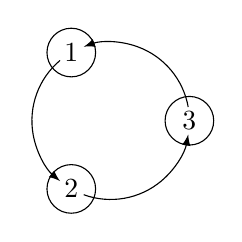
\begin{tikzpicture}
		\def \n {3}
		\def \radius {1cm}
		\def \margin {10} % margin in angles, depends on the radius
		
		\foreach \s in {1,...,\n}
		{
			\node[draw, circle] at ({360/\n * (\s - 3)}:\radius) {$\s$};
			\draw[->, >=latex] ({360/\n * (\s - 1)+\margin}:\radius) 
			arc ({360/\n * (\s - 1)+\margin}:{360/\n * (\s)-\margin}:\radius);
		}
		\end{tikzpicture}
	\end{figure}

	This means $1$ permutes to $2$, $2$ to $3$ and $3$ to $1$. An easy and rather not cumbersome notation we tend to work with is the cyclic notation, which is as follows:
	$$( 1 \: 2 \: 3  ),$$
	which we will work with in the remainder of this course.
\end{remark}

\begin{example}[Product of Permutations]
	Suppose we are dealing with the product of
	$$( 1 \: 4 \: 5 \: 2  ) [ ( 3 \: 4 \: 1  ) ( 2 \: 5 )  ]  . $$
	The order of operations is to be read backwards. Therefore, we deal with the square bracket first, then go ``forward'' to the first bracket. Take the element $1$ first; the permutation is as follows:	
	$$ 1 \to 3 $$
	so we first write $(1 \: 3 $. Then, starting with $3$,
	$$3 \to 4 \to 5 $$
	so we then write $(1 \: 3 \: 5$. Then, starting with $5$,
	$$ 5 \to 2 \to 1$$
	which means we are done---we have 1 cycle. Therefore, we close the bracket, $(1 \: 3 \: 5)$.
	
	Then we verify if $2$ and $4$ are independent cycles, or jointly form a $2$-cycle:
	$$\begin{aligned}
	&2 \to 5 \to 2 \\
	& 4 \to 1 \to 4 
	\end{aligned}$$
	therefore, these elements form $1$-cycle with itself. We denote the entire product as the set of permutations
	$$ (1 \: 3 \: 5)(2)(4).  $$
\end{example}

\begin{proposition}
	Permutations and matrices are both bijective objects. We have a \textbf{permutation matrix} defined as 
	$$ P = \sum_i e_{p(i), i}, $$
	where we can switch the positions of elements by imposing $e_{i,j}=1$.
\end{proposition}

This concludes a brief review of linear algebra. We will work largely with groups, rings, and perhaps fields in the following sections.


\section{Groups}

This is the easiest object of great complexity to study. Much of the course will be devoted to this.

\begin{definition}
	A \textbf{law of composition} on a set $S$ is any rule for combining pairs $a,b \in S$ to get another element in $S$.
\end{definition}

\begin{corollary}
	A more formal definition of law of composition is
	$$S \times S \to S, $$
	where $S \times S $ denotes the \textbf{product set}.
\end{corollary}

\begin{remark}
	There are many function operators we can use to denote multiplication:
	$$p=ab,a \times b, a \circ b,$$
	but in this course we will mostly be defining a law of composition by ourselves, so we will work with the notation $ a R b$ to indicate some law of composition $R$.
	
	Addition, of course, follows the notation $a+b$. 
\end{remark}

\begin{properties}
	\begin{enumerate}[noitemsep]
		\item With the multiplicative notation, a law of composition is \textbf{associative} if the rule
		$$(ab)c = a(bc) $$
		holds $\forall a,b,c \in S$.
		
		\item A law of composition is \textbf{commutative} if the rule
		$$ab=ba$$
		holds $\forall a,b,c \in S$. Groups whose elements are commutative are \textbf{abelian}.
	\end{enumerate}
\end{properties}

\begin{obs}
	Note that the associative law is more fundamental, because compositions of functions is associative. Let's see this with an example: suppose there exists a set $T$, and let $f$ and $g$ be maps from $T \to T$. As such,
	$$ g , f \leadsto  g \circ f  $$
	and it is easy to observe that this law of composition is associative. 
\end{obs}

\begin{definition}
	A \textbf{multiplication table} represents the law of composition on a particular set of elements of maps $T \to T$. Note that the table is to be read this way:
	
	$$\begin{array}{ c | c c c c}
	  & \: & \: & f & \: \\
	 \hline
	   & & & \vdots & \\
	  	  & & & \vdots & \\
	  	  	g  & \dots & \dots & g \circ f & \\
	  	  		  & & & & \\
	\end{array}$$
\end{definition}

\begin{proposition}
	Let an associative law of composition be given on a set $S$. There is a unique way to define a product of $n$ elements, $a_1, \dots, a_n$, for any integer $n$. We denote this by $[a_1 \dots a_n]$, with the following properties:
	\begin{enumerate}[  label=(\roman*)]
		\item The product $[a_1]$ of one element is the element itself.
		\item The product $[a_1 \: a_2]$ of two elements is given by the law of composition.
		\item For any $i \in [1,n), i\in \mathbb{N}$, $[a_1 \dots a_n] = [a_1 \dots a_i] [a_{i+1} \dots a_n]$.
	\end{enumerate}
\end{proposition}

\begin{proof}
	We can prove this by inducting on $n$. 
\end{proof}


\subsection{Group and Subgroups}

\begin{definition}
	A \textbf{group} is a set $G$ with a law of composition, satisfying the following properties:
	\begin{enumerate}[noitemsep]
		\item \textit{Associativity}: $\forall a,b,c \in G$, $(ab)c = a(bc)$.
		\item \textit{Identity}: there is an identity element $1$ or $e$,such that $ea=a$, $a=ea$, $\forall a \in G$.
		\item \textit{Inverse}: $\forall a \in G$, then there exists an element $b$ such that $ab = ba = 1$.
	\end{enumerate}
\end{definition}

\begin{definition}
	A subset $H$ of group $G$ is a \textbf{subgroup} if the following properties are satisfied:
	\begin{enumerate}[noitemsep]
		\item \textit{Closure}: $a,b \in H$ then $ab \in H$.
		\item \textit{Identity}: $1 \in H$.
		\item \textit{Inverse}: $a \in H \implies a^{-1} \in H$.
	\end{enumerate}
\end{definition}

It does not make sense to define subgroups without specifying the types of groups that we will be working with. In particular, we will examine a few types of groups in this class. The first is \textit{symmetric group}, ie. the group with composition operation that allows one to transpose/permute elements. We denote \textit{the symmetric group of order\footnote{To be defined later.} $n$ as $S_n$}.

\begin{remark}
	$S_n$ is nonabelian for $n\geq 3$. This is perhaps why $S_3$ is so interesting to study: any composition of elements in $S_3$ can be tricky.
\end{remark}

To make studying $S_3$ easier, the multiplication table of $S_3$ is as follows:
$$\begin{array}{c | c c c c c c}
	\circ & e & (123) & (321) & (12) & (23) & (13) \\
	\hline
	e & e & (123) & (321) & (12) & (23) & (13) \\
	(123) & (123) & (321) & e & (13) & (12) & (23) \\
	(321) & (321) & e & (123) & (23) & (13) & (12) \\
	(12) & (12) & (23) & (13) & e & (123) & (321) \\
	(23) & (23) & (13) & (12) & (132) & e & (123) \\
	(13) & (13) & (12) & (23) & (123) & (321) & e \\
\end{array}$$

Some other groups we will use often are
\begin{enumerate}[noitemsep]
	\item \textit{General linear group}: $\GL{n}{\R} = \condset{ M \in \Ma_{n \times n}}{\det M}{\neq}{0}$
	\item \textit{Special linear group}: $\SL{n}{\R} = \condset{ M \in GL_n (\R)}{ \det M }{=}{ 1} $
\end{enumerate}

Of course, we are always ready to study \textit{number groups}; we will focus on $\Z$, $\R$, $\Com$.

\subsection{Additive Group of Integers}

In general, when we refer to group of integers $\Z$, we refer to $(\Z, +)$. Why? Because we do not have multiplicative inverses in $\Z$ (except for $1$ and $-1$); think $1/2 \notin \Z$. In what follows, we denote additive group of integers as $\Z^+$. It turns out that this is an interesting group to study, not the least of which because it is quite tractable to do so. The only theorem/result we will prove is as follows.

\begin{theorem}
	Let $S \subset (\Z,+)$ be a subgroup (ie. $S \leq \Z$). Then \textit{either}
	\begin{enumerate}[noitemsep]
		\item $S = \{0\}$
		\item $S = \Z a$, $a$ is the smallest positive integer contained in $S$.
	\end{enumerate}
\end{theorem}

Before we prove the theorem, we need a lemma.

\begin{lemma}[Division]
	If $a\in \Z$, $n \in \Z$, and $a>0$, then $\exists q,r \in \Z \suchthat$
	$$ n = qa + r, \quad 0 \leq r < a $$
\end{lemma}

\begin{proof}
	Let $q$ be the largest integer such that $qa \leq n$. Let $r = n -qa \implies r \geq 0$. We now proceed to prove the second inequality by contradiction. Suppose $r \geq a$. Then, $ n - qa \geq a \implies (q+1)a \leq n $, which implies that $q$ is the largest integer. Hence, $r < a$.
\end{proof}

Now we're ready to prove the result.

\begin{proof}
	Suppose $S \leq \Z$.
	\begin{enumerate}[noitemsep]
		\item Then $0 \in S$ because it is the identity element in $S$. If this is the \textit{only element in $S$}, then $S= \{0\}$ is the trivial subgroup.
		\item If $0$ is not the only element of $S$, then $\exists n \in S, n \neq 0 \suchthat n>0$ or $-n>0$, and $n,-n \in S$. By well-ordering principle, then $S$ contains a least positive integer $n$. We claim both inclusions to prove $S=\Z a$.
		
		\begin{enumerate}
			\item[$\uline{(S \subset \Z a)}$] Let $n \in S$. Then by division lemma, $\exists q, r \in \Z$, $0 \leq r < a \suchthat n=qa+r$. Then, $n + (-qa) = qa +r + (-qa) = r \in S$. Since both $n$ and $qa$ are in the set $S$, and $r<a$, then this implies $r=0$ ($r$ is not positive). So $n = qa \in S$. Since this is true for every $n \in S$, this means $S \subset \Z a$.
		
			\item[$\uline{(S \supset\Z a )}$] This is slightly easier. Let $k \in \Z a$. Then $\Z a$ contins the smallest positive integer, and $ka = \underbrace{a+ a + \dots + a}_{k \text{ times}}$. Its inverse, $-ka \in S$ as well. Finally, $0 \in S \implies 0a \in S$, so $S$ is a subgroup, ie. $\Z a \subset S$.
		\end{enumerate}
	\end{enumerate}
as desired.
\end{proof}

\begin{definition}
	We call $\Z a + \Z b$ the \textbf{subgroup generated by $a$ and $b$.}
\end{definition}

\subsection{Cyclic Groups and Subgroups}

\begin{definition}
	If $x \in G$ and $G$ is a group, let $n \in \Z_+$, and $x^n = \underbrace{x \cdot x \cdot \dots \cdot x}_{n \text{ times}}$. Let $x^0 = e$. Then,
	$$ \cyclic{x} = \{ \dots , x^{-3}, x^{-2}, x^{-1}, e , x, x^2, x^3, \dots \} $$
\end{definition}

\begin{remark}
	$e = 1$ in the case of cyclic subgroups.
\end{remark}

\begin{remark}
	Exponentiation in group can yield the same elements. Because we are working with \textit{sets of elements}, we \textit{can} omit the elements that are repeated.
\end{remark}

\begin{properties}
	$\forall r,s, n \in \Z$, then
	$$\begin{aligned}
	x^{r+s} &= x^r x^s \\
	x^{rs} &= (x^r)^s	\\
	(x^{-1})^{n} &= (x^n)^{-1}
	\end{aligned}$$
\end{properties}

\begin{definition}
	The \textbf{order of a group $G$} is the number of elements in $G$, ie. $\abs{G}$. 
\end{definition}

\begin{definition}
	The \textbf{order of an element $x \in G$} is the smallest positive integer $n \suchthat x^n = 1$.
\end{definition}

\begin{definition}
	We say a group $G$ is \textbf{cyclic} if $\exists x \in G \suchthat G=$ cyclic subgroup generated by $x$, ie. $G =\cyclic{x} $.
\end{definition}

We now encounter an important proposition.

\begin{proposition}
	\label{propcyclicassubgroupofZ+}
	Let $\cyclic{x} \leq G$, where $x \in G$. Let $S = \condset{k \in \N}{x^k}{=}{e}$.
	\begin{enumerate}
		\item $S \leq \Z^+$.
		\item $x^r = x^s $ with $r \geq s$ are equal iff $x^{r-s} = e$, ie. iff $r - s \in S$.
		\item Suppose $S$ is not the trivial subgroup. Then $S = \Z n$ for some $n\in \N$, and $\set{1,x,x^2,\dots,x^{n-1}}$ are distinct elements of the subgroup $\cyclic{x}$. Obviously, the order of $\cyclic{x}$ is $n$.
	\end{enumerate}
\end{proposition}


\begin{proof}
	\begin{enumerate}
		\item Let $k, l$ be such that $x^k = x^l = e$, then $x^{k} x^{l} = x^{k+l} = e$, hence $k, l \in S$. This shows closure. Obviously, $x^0 = e$. Finally, if $x^k = e$, then $x^{-k} =(x^{k})^{-1} = e$. This shows inverse.
		
		\item This follows from cancellation law.
		
		
		\item Since all subgroups of $\Z^+$ are either trivial or of the form $\Z a$, $S = \Z n$ for some $n \in \N$. Since $k$ is arbitrary, divide $k$ by $n$, so we write $k = qn + r$ where $r$ is the remainder. Note that $x^{qn} = e^q = e$, and $x^k = x^{qn} x^{r}  =x^r$, so $x^k$ is equal to one of the elements in $\set{1,x,x^2,\dots,x^{n-1}}$. By the previous part, these elements are all distinct, because $x^n$ is the smallest positive power equal to $e$.
	\end{enumerate}
This concludes the proof.
\end{proof}


\subsection{Homomorphism}

\begin{definition}
	A \textbf{homomorphism} $f: G \mapsto H$, $(G,\star),(H,\ast)$ are groups, is defined $\forall a , b \in G$
	$$f(a \star b) = f(a) \ast f(b).$$
\end{definition}

\begin{example}
		Absolute value functions, exponentiation in $\R$, complex numbers, linear transformations, and determinants are all examples of homomorphisms.
\end{example}

\begin{example}
	There are two examples that are \textit{always true}, for any groups $G,H$ and homomorphism $f:G\mapsto H$:
	\begin{enumerate}[noitemsep]
		\item Take $f(g) = e_H$. This is the \textit{trivial homomorphism}.
		\item In particular, if $H \leq G$, then $i : H\mapsto G$ is called \textit{inclusion homomorphism of $G$ into $H$} if $i(h) = h$.
	\end{enumerate}
\end{example}

\begin{proposition}[Properties of Homomorphism]
	\label{proppropertiesofhomomorphism}
	For any groups $G,H$ and homomorphism $f:G\mapsto H$:
	\begin{enumerate}[noitemsep]
		\item $\forall a_1,a_2,\dots, a_k \in G$, $k \in \Z_+$, $f(a_1 a_2 \dots a_k) = f(a_1) f(a_2) \dots f(a_k)$. 
		\item $f(e_G) = e_H$.
		\item $\forall a \in G$, $f(a^{-1}) = [f(a)]^{-1}$.
	\end{enumerate}
\end{proposition}

\begin{proof}
	\begin{enumerate}
		\item Follows from induction on $n$.
		
		\item By the definition of homomorphism: note that
		\begin{align*}
			f(e_G) f(e_G) = f(e_G e_G) = f(e_G)
		\end{align*}
		and by cancellation law we then have $f(e_G) =e_H$.
		
		
		\item By definition, for every $a \in G$, $a^{-1} \in G$. Then, notice that
		\begin{align*}
		e_H = f(e_G) = f(a^{-1} a) = f(a^{-1}) f(a)
		\end{align*}
		premultiply $[f(a)]^{-1}$ on both sides gives the result.
	\end{enumerate}
	This concludes the proof.
\end{proof}

\begin{definition}
	The \textit{image of homomorphism $f: G \mapsto H$} is defined as
	\begin{align}
	\label{defimagehomomorphism}
	\im f = \condset{h \in H}{ f(g) = h}{, \: \forall h \in H}{, \: g \in G }
	\end{align}
\end{definition}

\begin{definition}
	The \textit{kernel of homomorphism $f: G \mapsto H$} is defined as
	\begin{align}
	\label{defkernelf}
	\ker f = \condset{g \in G}{ f(g) = e_H}{, \: \forall }{ g \in G }
	\end{align}
\end{definition}

There are some important results to remember and prove (by first principles).

\begin{proposition}
	Let $f: G \mapsto H$ be a homomorphism. Then,
	\begin{enumerate}[noitemsep]
		\item $\im f$ forms a \textit{subgroup of $H$}.
		\item $\ker f$ forms a \textit{subgroup of $G$}.		
	\end{enumerate}
\end{proposition}

\begin{proof}
	Check both by using the definition of subgroup: closure, identity, inverse
\end{proof}

Just like with functions, homomorphisms do not necessarily need to have good properties---in particular, as maps, they do not have to be injective or surjective. However, these properties are extremely nice to have, and give rise to good properties, which we will explore in later chapters. 

\begin{proposition}
	Let $f: G \mapsto H$ be a homomorphism. Then,
	\begin{enumerate}[noitemsep]
		\item $f$ is \textit{surjective/onto} $\iff$ $\im f =H$.
		\item $f$ is \textit{injective/one-to-one} $\iff$ $\ker f =\{e_G\}$.
	\end{enumerate}
\end{proposition}

\begin{remark}
	Instead of saying an injective map, we sometimes use \textit{embedding} instead.
\end{remark}


\begin{proposition}
	Let $f: G \mapsto H$ be a homomorphism. Then $K = \ker f$ is a subgroup of $G$.
\end{proposition}

\begin{proof}
	It suffices to prove that the kernel is non-empty and closed under products and inverses.
\end{proof}


\begin{proposition}
	Let $f: G \mapsto H$ be a homomorphism from $G$ to $H$ and let $K = \ker f$. Let $a,b \in G$. The following conditions are equivalent:
	\begin{enumerate}[noitemsep]
		\item \label{1} $f(a) = f(b)$
		\item \label{2} $a^{-1} b \in K$
		\item \label{3} $b \in aK$
		\item \label{4} $bK = aK$
	\end{enumerate}
\end{proposition}

\begin{proof}
	We proceed by showing that $(\ref{1}) = (\ref{2})$, and $(\ref{2}) \implies (\ref{4}) \implies (\ref{3}) \implies (\ref{2})$.
	
	Suppose (\ref{1}) is true. Then, $f(a) = f(b)$ implies, by properties of homomorphism,
	$$\begin{aligned}
	f^{-1} (a) f(a) &= f^{-1}(a)  f(b) \\
	\implies f(a^{-1} a ) &= f(a^{-1}b) \\
	\implies f( e_{G} ) &=f(a^{-1}b) \\
	\implies e_{H} &= f(a^{-1}b) \\
	\end{aligned}$$
	and the definition of kernel is
	$$ \ker f = \{ g \in G \mid f(g) = e_H \} $$
	so the last line can be written as $(\ref{2})$.
	
	Of course, $(\ref{2})$ is equivalent to $(\ref{1})$. We can rewrite the statement as
	$$ a^{-1} b \in \{ g \in G \mid f(g) = e_H \} $$
	and tracing back our steps yield the calculations
	$$\begin{aligned}
	\implies f(a^{-1} b ) &= e_H =  f( e_{G} ) \\
	\implies a^{-1} b &\in e_G \\
	\implies b &\in a \\
	\therefore f(b) &= f(a)
	\end{aligned}$$
	
	Let's show that $(\ref{2}) \implies (\ref{4})$. We use the fact that $(\ref{1}) = (\ref{2})$ established above, and make a couple of computations:
	$$ \begin{aligned}
	\forall x \in K, \quad bx &= a\underbrace{a^{-1}b}_{\in K} x = ax \in aK
	\end{aligned} $$
	so $bK \subset aK$. To show the other inclusion, we say that
	$$\begin{aligned}
	\forall x \in K, \quad ax &= b\underbrace{b^{-1}a}_{\text{inverse of } a^{-1}b } x = bx \in bK
	\end{aligned}$$
	and we know such inverse must exist by property of $(\ref{2})$, and must be an element of $K$. Hence, $aK \subset bK$.
	
	Now, we need to show that $(\ref{4}) \implies (\ref{3})$. We need to note that $k^{-1} k', \: \: k, k' \in K$ is \textit{not} the identity element. If we take $k, k'$ s.t.
	$$ bk = ak', \quad \forall k,k' \in K, $$
	then we can say
	$$\begin{aligned}
	b&= a \underbrace{k' k^{-1} }_{\in K} = a\bar{k}, \quad \forall \bar{k} \in K 
	\end{aligned}$$
	hence this can be written as $b \in aK$.
	
	Finally, we just need to show that $(\ref{3}) \implies (\ref{2})$. This is easy; by definition,
	\begin{align*}
	b &= ak \quad \forall k \in K \\
	\implies a^{-1} b &= k \quad \forall k \in K \\
	\therefore a^{-1} b &\in K
	\end{align*}
	as desired.
\end{proof}

We will circle back to this proposition once we learn more about cosets.

\subsection{Isomorphism and Normal Subgroups}

It might make no sense (at first) to talk about these two ideas in conjunction, but we hope that this will be a little clearer. We need to define a couple of things.

\begin{definition}
	Let $G$ be a group. Then $\forall a,g \in G$, the \textbf{conjugate of $a$ by $g$} is given by $gag^{-1}$.
\end{definition}

\begin{definition}
	If $N$ is a \textbf{normal subgroup} of $G$, denoted $N \lhd G$, then $\forall a \in N, g\in G$, $gag^{-1} \in N$.
\end{definition}

\begin{definition}
	Let $f: G \mapsto H$ be a \textit{bijective} homomorphism. Then $f$ is an \textbf{isomorphism}.
\end{definition}

\begin{proposition}
	If $f: G \mapsto H$ is an isomorphism, then $f^{-1}: H\mapsto G$ is also an isomorphism.
\end{proposition}

\begin{proof}
	The proof is constructive and pedagogically friendly. Take any $a,b \in H$. We need to verify two things:
	\begin{enumerate}[  align=left]
		\item[\uline{Bijectivity:}] $f^{-1} (a) = g$ $\forall g \in G$, meaning the inverse of a bijective map is bijective.
		\item[\uline{Homomorphism:}] Check if $f^{-1} (ab) = f^{-1} (a) f^{-1} (b)$. We perform the following calculations; let
		$$\begin{aligned}
		x&= f^{-1} (a) \\
		y&= f^{-1} (b)	\\	
		z&= f^{-1} (ab)
		\end{aligned}$$
		then $a=f(x)$, $b=f(y)$, $ab=f(z)$ (this operation is well-defined because we have a bijective homomorphism). Hence,
		$$f(xy) = f(x) f(y) = ab = f(z)$$
		using injectivity, $xy=z$, hence $f^{-1} (ab) = f^{-1} (a) f^{-1} (b)$.
	\end{enumerate}
This concludes the proof.
\end{proof}

\begin{definition}
	If $G$ and $H$ are \textbf{isomorphic}, then there exists an isomorphism $f: G \mapsto H$ (and the other direction is also defined). Notation-wise, we write $G \approx H$, or $f: G \overset{\approx}{\longmapsto} H $.
\end{definition}

\begin{remark}
	If $G$ and $H$ are groups, and are isomorphic (to each other), then all group theoretic properties are the same. In other words, these include, but not limited to,
	\begin{enumerate}[noitemsep]
		\item $\abs{G} = \abs{H}$
		\item $G$ cyclic $\iff$ $H$ cyclic
		\item $G$ abelian $\iff$ $H$ abelian
		\item $K$ is a subgroup (normal/cyclic) and $f: G \overset{\approx}{\longmapsto} H $, then $f(K)$ is a subgroup (normal/cyclic) of $H$.
	\end{enumerate}
\end{remark}

\begin{proposition}
	If $G$ and $H$ are cyclic groups, and $\abs{G} = \abs{H}$, then $G$ and $H$ are isomorphic.
\end{proposition}

Why do we care about isomorphisms? One of the motivational problems to the study of isomorphism is to classify different looking groups, but which are actually the same.

\begin{definition}
	If $G$ is a group, then the set of groups that are isomorphic to $G$ forms the \textbf{isomorphism class of $G$}.
\end{definition}

\begin{definition}
	An isomorphism from (group) $G$ to $G$ is called an \textbf{automorphism}.
\end{definition}

\begin{remark}
	The identity map is an automorphism, but it is often \textit{not} the only one. In particular, for all nonabelian groups, there always exists a nontrivial automorphism. In particular, conjugation is an automorphism.
\end{remark}

\begin{theorem}
	\label{thmconjugacyisautomorphism}
	Let $\gamma_x (g) = xgx^{-1}$ (a map $\gamma_x : G \mapsto G$). This map is an automorphism.
\end{theorem}

\begin{proof}
	This map is obviously a homomorphism. Equally obviously, $h = xgx^{-1} \iff g = x^{-1} hx$, so an inverse $\gamma_{x^{-1}}$ exists! As such, $\gamma_x$ is an isomorphism from itself to itself.
\end{proof}

\begin{remark}
	An \textit{injective homomorphism} is called an \textit{embedding}, denoted $f: G \hookrightarrow H$. Explicitly, this means $f$ is an isomorphism defined $f: G \to f(G)$, where $f(G) \subset H$.
\end{remark}

\begin{proposition}
	Let $\varphi: G \mapsto H$ be a group homomorphism. Then $\ker \varphi$ is a normal subgroup of $G$.
\end{proposition}

\begin{proof}
	We know that $\ker \varphi \leq G$. Let $k \in \ker \varphi$, and $x \in G$. Then,
	$$\begin{aligned}
	\varphi (x k x^{-1}) &= \varphi (x) \varphi (k) \varphi ( x^{-1})  \\
	&= \varphi (x) \varphi (x^{-1}) \\
	&= \varphi (x) [\varphi (x)]^{-1} \\
	&= e_H	
	\end{aligned}$$
	so $x k x^{-1} \in \ker \varphi$. Hence, $\ker \varphi \lhd G$.
\end{proof}

\subsection{Equivalence Relation and Partitions}

\begin{definition}
	An \textbf{equivalence relation} $\sim$ is a relation that satisfies three properties:
	\begin{enumerate}[noitemsep]
		\item \textit{Reflexive}: $\forall a \in S$, $a \in a$
		\item \textit{Symmetric}: $\forall a,b \in S$, if $a \sim b$, then $b \sim a$
		\item \textit{Transitive}: $\forall a,b,c \in S$, if $a \sim b$ and $b \sim c$, then $a \sim c$.
	\end{enumerate}
\end{definition}

\begin{remark}
	Group isomorphism is an \textit{equivalence relation}.
\end{remark}

\begin{example}
	Take $x,y \in \Z$. Let $\sim $ be a relation defined
	$$ x \sim y \iff x-2y = 2n, \: \: n \in \Z $$
	then $\sim $ is an equivalence relation.
	\begin{enumerate}[noitemsep]
	\item \textit{Reflexive}: $\forall a \in S$, $a \in a$. In particular, $x - x = 0 = 2(0)$.
	\item \textit{Symmetric}: $\forall a,b \in S$, if $a \sim b$, then $b \sim a$. In particular, $x - y = 2n \implies y - x = -2n$. Hence, $x \sim y \implies y \sim x$.
	\item \textit{Transitive}: $\forall a,b,c \in S$, if $a \sim b$ and $b \sim c$, then $a \sim c$. In particular,
	$$ x \sim z = (x - y) + (y - z) = x -z \quad (= 2n + 2n = 4n \in 2\Z)  $$
	\end{enumerate}	
\end{example}

We now prove a really important theorem in equivalence relation, vis-\`a-vis \textit{partitions}.

\begin{definition}
	A \textbf{partition} of set $S$ is a way of subdividing $S$ into nonempty, nonoverlapping subsets. In particular,
	$$S = S_1 \cup S_2 \cup \dots \cup S_n$$
	where every element of $S$ is contained in exactly one subset $S_i$.
\end{definition}

\begin{theorem}
	Equivalence relation on set $S$ and partitions on $S$ are one-to-one correspondent.
\end{theorem}

We prove this in two propositions.

\begin{proposition}
	Every partition of set $S$ corresponds to an equivalence relation.
\end{proposition}

\begin{proof}
	Let $S= S_1 \cup S_2 \cup \dots $. Let $\sim$ be an equivalence relation on $S \suchthat \forall x,y \in S$, $x \sim y \iff \exists i \in \N \suchthat x,y \in S_i$.
	\begin{enumerate}[noitemsep]
		\item \textit{Reflexive}: $\forall a \in S$, $a \in a$. In particular, $x,x \in S$.
		\item \textit{Symmetric}: $\forall a,b \in S$, if $a \sim b$, then $b \sim a$. In particular, $\exists i \in \N \suchthat x , y \in S_i$. Then $y \sim x$ follows.
		\item \textit{Transitive}: $\forall a,b,c \in S$, if $a \sim b$ and $b \sim c$, then $a \sim c$. In particular, $a, b \in S_i$, $b,c \in S_j$. But $b \in S_i \cap S_j$. Since we imposed that $i \neq j$, and partitions by definition are nonoverlapping, $S_i = S_j$. Hence, $x,y,z \in S_i$, so $x \sim z$.
	\end{enumerate}		
	so partitions correspond to an equivalence relation.
\end{proof}

\begin{proposition}
	Every equivalence relation defined on $S$ induces a partition on $S$.
\end{proposition}

We will need the following definition to prove the proposition directly above.

\begin{definition}
	If $\sim $ is an equivalence relation on $S$, and if $a \in S$, then we define the \textbf{equivalence classes} of $a$ to be the set
	$$ E_a = \condset{b \in S}{b}{ \sim}{ a}$$
\end{definition}

\begin{proof}
	In particular, we want to show that every equivalence relation defined on $S$ induces equivalence classes on $S$, and these are partitions on $S$. We need to prove three things:
	\begin{enumerate}%[noitemsep]
		\item $\uline{\bigcup_{i \in \N} E_i = S}$. This is easy to show, since, by reflexivity, $a \in E_a$ is guaranteed (hence each equivalence class is nonempty). And, obviously, $\bigcup_{a \in S} [a] \in S$
		\item  \uline{Nonempty}. Explained above.
		\item \uline{Nonoverlapping}. We show the contrapositive: that if $E_a$ and $E_b$ have an element in common, then $E_a = E_b$. In particular, take $c \in E_a \cap E_b$. Then $c\sim a $ and $c \sim b$, then $a\sim b$. This means that $\forall x \in E_a$, then by definition, $x \sim a$ and $a \sim b$ implies $x \sim b$ by transitivity; $x \in E_b$, so $E_a \subset E_b$.
		
		In the same way, we say that $\forall y \in E_b$, $y \sim b$, and $b \sim a$ implies $y \sim a$, by transitivity. This means that $y \in E_a$, so $E_b \subset E_a$.
	\end{enumerate}
	So we've proven both inclusions, hence equivalence classes form partitions on $S$.
\end{proof}

\begin{definition}[Equivalence classes of modulo $\sim$]
	If $\sim$ is an equivalence relation on $S$, we let $S/\sim $ or $\bar{S}$ (which reads $S \mod \sim$) be the set of equivalence classes of $\sim$.
\end{definition}

\begin{example}
	Define $\sim$ as the integer relation $x \sim y \iff x - y \equiv 0 \mod 2$. Then this defines a set of equivalence classes on the integers, denoted $\overline{\Z}$. In particular, it admits elements of both parity, ie.
	$$ \overline{\Z}  = \{ \{2n \} , \{ 2n+ 1\}   \} \quad \forall n \in \Z$$
	but this notation needs some refinement: it is a little tedious to refer to sets of sets. If we want to emphasise a particular element of the set $E$---to refer to a set as an element---we use the notation $[A]$. In particular, we can say that
	$$ \overline{\Z}  = \{ [2n] , [2n+1]  \} \quad \forall n \in \Z$$
\end{example}

\begin{remark}
	There are generally a lot of ways to represent the same set of equivalence classes. For example,
	$$ \overline{\Z} = \{ \overline{0}, \overline{13} \} = \{ \overline{391}, \overline{24} \} = \dots $$
\end{remark}

\begin{example}
	Let us illustrate a particular map.
	
	\begin{figure}[H]
		\centering
			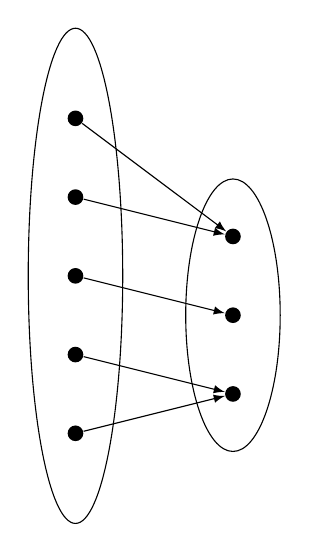
\begin{tikzpicture}
		%put some nodes on the left
		\foreach \x in {1,2,3,4,5}{
			\node[fill,circle,inner sep=2pt] (d\x) at (0,\x) {};
		}
		\node[fit=(d1) (d2) (d3) (d4) (d5),ellipse,draw,minimum width=1.2cm] {}; 
		%put some nodes on the center
		\foreach \x[count=\xi] in {1.5,2.5,3.5}{
			\node[fill,circle,inner sep=2pt] (r\xi) at (2,\x) {};
		}
		\node[fit=(r1) (r2) (r3),ellipse,draw,minimum width=1.2cm] {} ; 
		%put some nodes on the right
		\draw[-latex] (d1) -- (r1);
		\draw[-latex] (d2) -- (r1);
		\draw[-latex] (d3) -- (r2);
			\draw[-latex] (d4) -- (r3);
				\draw[-latex] (d5) -- (r3);
		\end{tikzpicture}
	\end{figure}
	
	Define this map $f:A \mapsto B$ as an equivalence relation on $A \suchthat x \sim y  \iff  f(x) = f(y)$. We skip the verification here. We want to focus on the characterisation of equivalence classes:
	$$ E_s = \condset{  r \in A }{f(r) }{=}{f(s)} $$
	which implies that the \textit{pre-images of $f(s)$}, $f^{-1} ( \{f(s)\} )$, is the set of elements of the equivalence class of $s$. So
	$$ \overline{A} = \{ f^{-1} ( \{f(a)\} ), f^{-1} ( \{f(c)\} ) , f^{-1} ( \{f(d)\} )  \} $$
	which is not \textit{\uline{the} representation of the entire set $A$}.
\end{example}

\begin{definition}
	A set of preimages of such $f: A \to B$ is called the \textbf{fiber} of $f$.
\end{definition}

Below is an important proposition for the class.

\begin{proposition}
	There exists a bijective correspondence between \textit{equivalence classes} and the \textit{image} of a map. In other words, if $f: A \mapsto B$ and $\sim$ as defined (an equivalence relation), then $\exists \varphi : \overline{A} \mapsto \im f$, where $\varphi$ is a bijection.
\end{proposition}

\begin{proof}
	If $x \in \im f $ and $x \overset{\psi}{ \longmapsto  }  [ f^{-1} ( \{x\} ) ] $, then we can define $ [E] \overset{\varphi}{\longmapsto } f(E)  $. Alternatively, we can always write $[E] = \overline{a}$ for some $a \in A$, and check that $\psi (a) = \varphi (\overline{a})$.
\end{proof}

\subsection{Cosets, Congruences, and Modulo Arithmetic}

A particularly useful objective that is used all the time in the coset.

\begin{definition}
	If $H \leq G$, and $a \in G$, the set 
	$$aH = \{ b \in G \mid b = ah \text{ for some } h \in H \} = \{  ah \mid h \in H \} $$
	is called the \textbf{left coset of $G$ in $H$}.
\end{definition}

\begin{proposition}
If $a, b \in G$, then we say $a$ is \textbf{congruent} to $b$ ($a \equiv b$) if $b = ah$ for some $h \in H$.
\end{proposition}

\begin{proof}
	We need to show that this is an equivalence relation.
	\begin{enumerate}%[noitemsep]
		\item \textit{Reflexive}: if $a \equiv a$, and $a = ah \implies h = e$.
		\item \textit{Symmetric}: if $a \equiv b$ then $b=ah$. Then, $bh^{-1} = a$ and $h^{-1} \in H$, so $b \equiv a$.
		\item \textit{Transitive}: if $a \equiv b \implies b = a h_1$ and $b \equiv c \implies c = b h_2$, then $c = b h_2 = a(h_1 h_2) \implies a \equiv c$.
	\end{enumerate}
	And the equivalence classes defined by such equivalence relation is
	$$\begin{aligned}
	E_a &= \{ b \in G \mid a \equiv b \} \\
	&= \{ b \in G \mid b = ah \text{ for some } h \in H \} \\
	&= \{ ah \in G \mid h \in H  \}
	\end{aligned}$$
	which is the left coset of $G$ in $H$. Therefore, the equivalence classes induced by congruence (which, as we checked, is an equivalence relation) are \textit{left cosets}.
\end{proof}

\begin{proposition}
	Let $G$ be a group, and $H \leq G$. Then, the left cosets of $H$ form partitions of $G$.
\end{proposition}

\begin{proposition}
	The cardinalities (orders) of any two cosets are equal.
\end{proposition}

\begin{proof}
	We can construct bijection $\varphi$ between cosets. Let $a \in G$. Then the map $\varphi_a : H \mapsto aH$ where $\varphi_a (h) = ah$ has an inverse. It is defined by $(\varphi_a)^{-1} (g) = a^{-1} g \: \: \forall g \in aH$ (remember $(\varphi_a)^{-1} =  \varphi_{a^{-1}}$ is defined as $(\varphi_a)^{-1} : aH \mapsto H$). As such, $\varphi_a (h)$ is a bijection, hence $\abs{H} = \abs{aH}$.
\end{proof}

This lets us establish the following proposition, which we call the counting formula.

\begin{proposition}[Counting formula]
	Let $H \leq G$. Since $\abs{H} = |aH|$, we can use the order of cosets of $H$ in $G$ to find the order of $G$. In particular,
	$$ \abs{G} = \abs{H} (\text{number of cosets of $H$ in $G$}) $$
\end{proposition}

\begin{definition}
	The number of cosets of $H$ in $G$ is called the \textbf{index of $H$ in $G$}.
\end{definition}

\begin{theorem}[Lagrange's Theorem]
	\label{lagrangethm}
	The order of any subgroup of group $G$ divides the order of $G$.
\end{theorem}

\begin{proof}
	Already established above. This is the direct consequence of the counting formula:
	$$ \abs{G} = \abs{H} [G: H] $$
	where $[G:H]$ is the number of (left) cosets of $H$ in $G$.
\end{proof}

\begin{remark}
	The reverse of Theorem \ref{lagrangethm} does not work. Take $S_4$, the symmetric group of order 4. Just because it has 24 elements \textit{does not mean} there is a subgroup of order 12. There can be divisors of $G$ that are \textit{not} the orders of subgroups of $G$.
\end{remark}

\begin{proposition}
	\label{primecyclic}
	Let $G$ be a group of order $p$, where $p>1$ is a prime number. Then $G$ is cyclic.
\end{proposition}

\begin{proof}
	Elements in such group $G$ has either order 1 or $p$. So, $\abs{G} \geq 2$ because $1$ is not a prime number. Therefore, $\exists $ a non-identity element $x \in G$. Hence, $\abs{\cyclic{x}} = p$, and $G= \cyclic{x} $.
\end{proof}

A particularly powerful interpretation comes when we talk about cosets in conjunction with equivalence classes. We note that the counting formula can be used to identify the following fact: that the left cosets of $\ker \varphi$ are the nonempty fibres of the map $\varphi$. Hence, there exists  abijective correspondence between fibres and the elements of the image. This implies
\begin{align*}
[G:\ker \varphi] = \abs{\im \varphi}
\end{align*}
A few results follow immediately.

\begin{corollary}
	\label{cororderskerimgroupsrelationship}
	Let $\varphi: G \to \GG$ be a homomorphism between finite groups. Then,
	\begin{enumerate}
		\item $\abs{G} = \abs{\ker \varphi} \abs{\im \varphi}$,
		\item $\abs{\ker \varphi}$ divides $\abs{G}$,
		\item $\abs{\im \varphi}$ divides $\abs{G}$ and $\abs{\GG}$.
	\end{enumerate}
\end{corollary}

\begin{proof}
	These proofs are elementary. We omit them here.
\end{proof}

\begin{remark}
	By definition, equivalence classes are fibers fo $f$, which are sets $f^{-1} ( \{y\})$, $y \in \im f$. There exists a bijection between cosets and fibers. In particular, we say that if $f : G \mapsto H$ is a homomorphism, and $K= \ker f$, then $\abs{G} = |\ker f\mid |\im f|$.
	
	Another observation from this is $|\im f|$ divides $\abs{G}$ (meaning $|\im f|$ is a factor of $\abs{G}$). Furthermore, since $\im f \leq H$, this implies $|\im f|$ divides $\abs{H}$.
\end{remark}

\begin{remark}
	If $\gcd (\abs{G},\abs{H}) = 1$, then $|\im f\mid = 1$. This implies $\im f \subset H$, so $\im f $ is a \textit{trivial subgroup of $H$}.
\end{remark}

Now, there is a particularly useful characterisation of index. We call this the \textit{multiplication index theorem}.

\begin{theorem}[Multiplication index theorem]
	\label{thmmultiplicationindexthm}
	Let $K \leq H \leq G$ (as groups; as sets, $K \subset H \subset G$). Then $[G:K] = [G:H] [H:K]$.
\end{theorem}

\begin{proof}
	The idea is as follows. If $H \leq G$, and $[G:H]=2$, then we can say that a coset takes up ``half'' of $G$. Of course, this is not well-defined if we are talking about infinite groups, so we refrain from doing so. In the finite case (ie. if orders of the groups are finite), this follows from applying the counting formula.
	
	In general, we prove the theorem as follows. Let $m \coloneqq [G:H]$ and $n \coloneqq [H:K]$. Suppose $m, n$ are finite. Then by definition of cosets, we can write both
	$$ \begin{aligned}
	G &= g_1 H \cup g_2 H \cup \dots g_m H \\
	H &= h_1 K \cup h_2 K \cup \dots h_n K \\	
	\end{aligned} $$
	where $g_i \in G $ and $h_i \in H$ $\forall i$. Then, $\forall g \in G$,
	$$ \begin{aligned}
	gH &= g \cup ( h_1 K \cup h_2 K \cup \dots h_n K  ) \\
	&= g h_1 K \cup g h_2 K \cup \dots g h_n K 
	\end{aligned} $$
	and we want to prove that these parts are still partitions.
	
	We proceed by contradiction. Pick $i \neq j \suchthat x \in g h_i K \cap g h_j K$. Then, $ g^{-1} x \in h_i K$ and $ g^{-1} x \in h_j K$. But we've assumed at first that $h_i K \cap h_j K = \emptyset$. Contradiction.
	
	Hence we can write
	$$\begin{aligned}
	G = ( g_1 h_1 K \cup g_1 h_2 K \cup \dots g_1 h_n K   ) &\cup ( g_2 h_1 K \cup g_2 h_2 K \cup \dots g_2 h_n K   ) \cup \dots \\
	& \dots \cup ( g_m h_1 K \cup g_m h_2 K \cup \dots g_m h_n K   )
	\end{aligned} $$
	so that $G$ has $m \times n$ cosets of $K$. Hence, $[G:K] = [G:H] [H:K] = mn$.
	
	We will prove the infinite case once we cover quotient groups.
\end{proof}

Until now, we've worked with \textit{left cosets}. We can and should work with right cosets.

\begin{definition}
	If $H \leq G$, and $a \in G$, the set 
	$$Ha = \{ b \in G \mid b = ha \text{ for some } h \in H \} = \{  ha \mid h \in H \} $$
	is called the \textbf{right coset of $G$ in $H$}.
\end{definition}

\begin{proposition}
	If $a,b\in G$, then $a,b $ are in the right coset $\iff$ $a \in Hb \iff ab^{-1} \in H$.
\end{proposition}

\begin{remark}
	In general, the left and right cosets of subgroup $H$ are \textit{different}.
\end{remark}

\begin{remark}
	Kernels are normal subgroups of homomorphisms.
\end{remark}

\begin{proposition}
	$H \lhd G \iff \forall  h \in H, \: \: hG = Gh$. To be more specific, let $H \leq G$. The following conditions are equivalent:
	\begin{enumerate}%[noitemsep]
		\item $H$ is normal
		\item $\forall g \in G$, $g H g^{-1} = H$
		\item $\forall g \in G$, $gH = Hg$ (the sets are equal)
		\item Every left coset is a right coset
	\end{enumerate}
\end{proposition}

The reason why we talk about cosets is so we can apply them to studying number theory, and, later, quotient groups.

\begin{definition}
	Let $a,b \in \Z$, $n \in \Z_{>0}$. Then, $a \equiv b \mod n \iff b - a = m(n)$ for some $m \in \Z_{>0}$.
\end{definition}

\begin{remark}
	We can use the notion of equivalence classes to perform construction of modulo classes of $a$, denoted $\overline{a}$. In particular,
	$$\begin{aligned}
	\overline{a} &= \{ b \mid b-a \in \Z n \} \\
	&= \{ a + k \mid k \in \Z n \} = a+ \Z n
	\end{aligned}$$
	so $\overline{a}$ is a coset of $\Z n$.
\end{remark}

\begin{remark}
	Note that
	$$\begin{aligned}
	\Z 10 = 10 \Z &= \{\dots, -10,0,10, \dots \} \\
	3 + \Z 10 &= \{ \dots, -7, 3, 13, \dots \} \\
	\implies a + \Z n &= \{  \dots, a-2n, a - n, a , a+ n, a+ 2n , \dots  \}
	\end{aligned}$$
	so $a + \Z n$ has $n$ many \textit{distinct cosets}, namely,
	$$ a + \Z n = \{ a, a + \Z 1,  a + \Z 2, \dots, a + \Z (n-1)  \} = \{ \overline{1}, \overline{2}, \dots, \overline{n-1} \}$$
	are the congruence classes of modulo $n$.
\end{remark}

\begin{definition}
	Operations on these cosets are as follows:
	\begin{enumerate}%[noitemsep]
		\item $\overline{a} + \overline{b} = \overline{a+b}$
		\item $  \overline{a} \cdot \overline{b} = \overline{a \cdot b}$
	\end{enumerate}
\end{definition}

\begin{remark}
	Note that this definition is not entirely ``error-proof''. Since there is generally no unique representation of equivalence classes, it calls for the following proposition.
\end{remark}

\begin{proposition}
	If $\overline{a} = \overline{a'}$ and $\overline{b} = \overline{b'}$, then $\overline{a+b} = \overline{a' + b'}$ and $\overline{ab} = \overline{a'b'}$.
\end{proposition}

\begin{proof}
	WLOG, $\forall r,s \in \Z$, let
	\begin{align*}
	a' &= a + rn \\ 
	b' &= b + sn \\ 
	\end{align*}
	then
	\begin{align*}
	a' + b' &= (a+ rn) + (b + sn) \\
	& = (a+b) + (r+s)n \\
	\implies \overline{a' + b'} &= \overline{a+b}
	\end{align*}
	Similarly,
	\begin{align*}
	a' b' &= (a+rn)(b+sn) \\
	&= (ab) + (as + br + srn) n \\
	\implies \overline{a'b'} &= \overline{ab}
	\end{align*}
	as desired.
\end{proof}

\begin{example}
	We show that these operations may not be well-defined in a particular scenario. Take modulo $6$. In particular, take congruence classes $\overline{1}$ and $\overline{5}$. Then, take
	$$ \begin{aligned}
	1 \cdot 5 = 5 &\equiv 5 \mod 6 \\
	7 \cdot 5 = 35 &\equiv 5 \mod 6	\\
	13 \cdot 11 = 143 &\equiv 5 \mod 6	
	\end{aligned} $$
	but the following operation:
	$$\forall a,b \in \Z, \overline{a} < \overline{b} \iff a < b$$
	is not well-defined; pick $13 \in \overline{1} $ and $5 \in \overline{5}$ to see why.
\end{example}

The reason why we defined multiplication and addition of cosets is because these operations are the same for the integers.
\begin{enumerate}%[noitemsep]
	\item Additive identity in modulo $n$: $\overline{0}$, which is analogous to $0$ in the integers.
	\item Multiplicative identity in modulo $n$: $1$, or $\Z / n\Z = 1 \mod n$. 
	\item Additive inverse in modulo $n$: $\overline{-a} = -a \mod n$.
\end{enumerate}
And we can use associativity in groups to show a number of results.

\begin{corollary}
	$(\Z / \Z n , + )$ is an abelian group.
\end{corollary}

\begin{proof}
	Show that this satisfies group properties, and commutativity.
\end{proof}

\begin{remark}
	$(\Z / \Z n , + )$ is a cyclic group generated by $\overline{1}$, with addition as operation.
\end{remark}


\subsection{Correspondence Theorem}
Now, we can, and will, describe a particular application of all the materials we have built. We set the scene as follows. Let $\varphi : G \mapsto \GG$ be a group homomorphism, and $H \leq G$. We can always restrict $\varphi$ to $H$, ie.
\begin{align*}
\varphi|_{H} :  H \mapsto \GG
\end{align*}
in particular, this is still a homomorphism (this is not hard to check at all), with the kernel being the intersection of $\ker \varphi$ with $H$:
\begin{align*}
\ker (\varphi|_H ) = \ker \varphi \cap H
\end{align*}
These facts are clear by definition. The image of the restriction is the same as $\im \varphi(H)$ (ie. image of $H$ under the map $\varphi$). By \colref{cororderskerimgroupsrelationship}, we have the obvious fact that $\abs{\im \varphi|_{H}} $ divides both $\abs{H}$ and $\abs{\GG}$; hence, if $\gcd(\abs{H},\abs{\GG}) =1$, then it is obviously true that $\varphi(H) = \set{e}$, so $H \in \ker \varphi$.


To make the ideas in this example more concrete, we introduce the following proposition---which adds another item to the list of properties of homomorphism.

\begin{proposition}
	\label{propsubgroupsrelationsinhomomorphism}
	Let $\varphi: G \mapsto \GG$ be a group homomorphism. Denote its kernel by $K$. Let $\HH \leq \GG$. Let $\varphi^{-1} (\HH) \coloneqq H$. Then,
	\begin{enumerate}
		\item $K \subset H \leq G$ (kernel is contained in $H$, while $H$ is a subgroup of $G$).
		\item if $\HH \lhd \GG$, then $H \lhd G$.
		\item if $\varphi$ is surjective, and $H \lhd G$, then $\HH \lhd \GG$.
	\end{enumerate}
\end{proposition}

\begin{proof}
	\begin{enumerate}
		\item This is simple enough to check, as long as we keep in mind that $\varphi^{-1}$ is not a map: by definition, the symbolic $\varphi^{-1} (\HH) = H$ is the preimage of $\HH$. Obviously, if $x \in \ker \varphi$, then $\varphi(x) =e$. Since $e \in \HH$, $x \in H$, then it follows that $H \supset K$ (since $K \leq H$). We leave the subgroup verification as an exercise.
		
		
		\item Let $\HH \lhd \GG$. Pick $h \in H$ and $g \in G$. Note that the image of the conjugate of $h$ by $g$ is $\varphi(ghg^{-1}) = \varphi(g) \varphi(h) \varphi(g)^{-1} = \varphi(h)$, ie. the conjugation results in the image of $h$. Obviously, by construction, $\varphi(h) \in \HH$. Since $\HH$ is normal, we then have $\varphi(ghg^{-1}) \in \HH$, implying $ghg^{-1} \in H$. 
		
		
		\item This should be intuitively true. To see why this is the case, pick $a \in \HH$ and $b \in \GG$. Then, $a = \varphi(x)$ and $b = \varphi(y)$ is guaranteed for some $x \in H$ and $y \in G$, by surjectivity of the map $\varphi$. In particular, since $H$ is normal, $yxy^{-1} \in H$, so $\varphi(yxy^{-1}) = \varphi(y) \varphi(x) \varphi(y)^{-1} = bab^{-1} \in \HH$.
	\end{enumerate}
This concludes the proof.
\end{proof}

The following is a profound connection between subgroups of domain and range of a group homomorphism.

\begin{theorem}[Correspondence Theorem]
	\label{thmcorrespondencetheorem}
	Let $\varphi: G \mapsto \GG$ be a surjective group homomorphism. Denote its kernel as $K$. There exists a bijective correspondence between subgroups of $\GG$ and subgroups of $G$ that contains $K$. We define the correspondence as
	\begin{align*}
	\text{a subgroup } H \text{ of } G \text{ that contains } K  \leadsto & \text{ its image } \varphi(H) \in \GG \\
	\text{a subgroup } \HH \text{ of } \GG  \leadsto & \text{ its preimage } \varphi^{-1} (\HH) \in G
	\end{align*}
	then,
	\begin{enumerate}
		\item if $H$ and $\HH$ are corresponding subgroups, then $H \lhd G \iff \HH \lhd \GG$.
		\item if $H$ and $\HH$ are corresponding subgroups, then $\abs{H} = \abs{\HH} \abs{K}$.
	\end{enumerate}
\end{theorem}


\subsection{Quotient Groups}
With the materials we have built, we can construct \textit{quotient groups}.

\begin{definition}
	Let $N \lhd G$. Furthermore, let $ \qgroup{G}{N} = \{ \text{ cosets of $N$ in $G$}  \}$. Let $x \in \qgroup{G}{N}$, which is represented as either $\overline{a}$ or $[aN]$. We can define a map $\pi : G \mapsto \qgroup{G}{N}$ where $\pi (a) = \overline{a}$, $\forall a \in G$.
\end{definition}

\begin{theorem}
	\label{derivativeOfFIT}
	There exists a law of composition on $\qgroup{G}{N}$ that makes it a group, with the properties that $\pi$ is a \textit{surjective homomorphism} with $\ker \pi = N$.
\end{theorem}

The fact that $\pi(a)$ is surjective shouldn't be surprising; a minute or two of staring should make this apparent. But we need to find such law of composition to make the theorem hold. We need a few results.

\begin{definition}
	If $A,B \leq G$, then we define $A \times B$ as the \textbf{product set}
	$$A \times B = \condset{(a \times b)}{a \in A, \: }{ b\in B}{} $$
\end{definition}

\begin{remark}
	The product set is \textit{generally not a subgroup of $A$ or $B$ unless there are some ``good'' properties with the subgroups}.
\end{remark}

\begin{lemma}
	If $N \lhd G$, and if $a,b \in G$, then $(aN)(bN) = (ab)(N)$.
\end{lemma}

\begin{proof}
	If $N$ is normal, then we have that $aN=Na$, $\forall a \in G$. Then,
	\begin{align*}
	(aN)(bN) &= (aN)(Nb) \\
	&= a (Nb) = a (bN) = (ab)N
	\end{align*}
	as desired.
\end{proof}

\begin{definition}
	\label{deflawofcompositionquotientgroup}
	Let the law of composition on $\qgroup{G}{N}$ be such that $\forall [c_1], [c_2] \in \qgroup{G}{N}$, $[c_1 c_2] = [c_1][c_2]$. By lemma, $c_1 c_2$ is in the coset of $N$, and $[c_1 c_2] $ is an element of $\qgroup{G}{N}$.
\end{definition}

\begin{proof}[Check: $\qgroup{G}{N}$ equipped with \defnref{deflawofcompositionquotientgroup} forms a group]
	We check all the conditions.
	\begin{enumerate}%[noitemsep]
		\item \uline{Associativity}: $\forall a,b,c \in \qgroup{G}{N}$,
		$$\overline{a} \overline{b} \overline{c} = \overline{ab} \overline{c} = \overline{(ab)c } = \overline{abc}$$
		
		\item \uline{Identity}: $\overline{1}$ is obviously the identity element.
		
		\item \uline{Inverse}: recall that $ \overline{a} \cdot \overline{a^{-1}} = \overline{a\cdot a^{-1}} = \overline{1}$ and $ \overline{a^{-1}} \cdot \overline{a} = \overline{a^{-1} \cdot a} = \overline{1}$.
	\end{enumerate}
This concludes the proof. 
\end{proof}

\begin{lemma}
	$\pi: G \mapsto \qgroup{G}{N}$ is a surjective homomorphism with $K= \ker \pi = N$.
\end{lemma}

\begin{proof}
	First, $\pi: G \mapsto \qgroup{G}{N}$ is indeed a homomorphism (check). Surjectivity requires us to check the image of the homomorphism, ie.
	\begin{align*}
	\im \pi  &= \condset{x \in \qgroup{G}{N}}{\exists g \in G \suchthat  \pi (g) }{ = }{x}  \\
	&= \condset{ x}{x }{\in}{ \qgroup{G}{N} } = \qgroup{G}{N}
	\end{align*}
	Also,
	\begin{align*}
	\ker \pi &= \condset{y \in G}{ \pi (y)}{ = }{e_{\qgroup{G}{N}} } \\
	&= \condset{y}{y}{\in}{N} = N
	\end{align*}
	as desired.
\end{proof}

With this, we can talk about a lot about integer groups---in particular, as we said before, every subgroup of the form $\Z n$, $n \in Z$, is normal in $(\Z, +)$. Therefore, we can define $G/ N = \Z / \Z n = \{ \overline{0}, \overline{1}, \dots, \overline{n-1} \}$. By Theorem \ref{derivativeOfFIT}, we can define $\varphi : \Z \mapsto \Z /n$ where $\varphi(a)= \overline{a} = \overline{a + \Z n}$\footnote{An equivalent notation I use is $[a]$.}. This is indeed a surjective homomorphism.

Let us see why normal subgroup is a really important criterion for Theorem \ref{derivativeOfFIT} to hold.

\begin{example}
	Let $G=(S_3,\circ)$. Define generators $x=(123)$ and $y=(12)$, and $\cyclic{x} $ is a normal subgroup of $G$ (check). Let us find the cosets (partitions) of the this generator: since $y$ is of order 2, $\cyclic{x}$ is index 2 in $G$. The cosets are
	$$\begin{aligned}
	1 \cyclic{x} &= \{ 1, x, x^2\} = \cyclic{x} 1 \\
	y \cyclic{x} &= \{ y, yx, y x^2 \} = \{ y, x^2 y, xy \} \\
	&= \cyclic{x} y
	\end{aligned}$$
	so $\cyclic{x}$ is indeed a normal subgroup of $G$. The quotient group $G / N = S_3 / \cyclic{x} = \{  1 \cyclic{x}, y \cyclic{x} \} = \{ \overline{1}, \overline{y}  \}$. In particular, because the order of the group is prime, we can use Proposition \ref{primecyclic} to say that $S_3 / \cyclic{x} \cong C_2$.
	
	We now check that $\cyclic{y}$ is \textit{not} a normal subgroup of $G$. Just use the fact that if $\cyclic{y}  \lhd S_3$, then $\forall g \in G$, $g y g^{-1 } \in \cyclic{y} $. But, take $x=(123)$ as defined above
	$$\begin{aligned}
	x y x^{-1} &= ( x(1) x(2) ) \\
	&= ( 23 ) \notin \cyclic{y} 
	\end{aligned}$$
	and, take $\qgroup{S_3}{ \cyclic{y}} = \{ [1,y], [x,xy], [x^2, x^2 y] \} = \{ \overline{1} , \overline{x}, \overline{x}^2 \}$:
	$$\begin{aligned}
	\{ 1,y \} \circ \{ x,xy \} &= \{ 1x, 1xy, yx, yxy \} \\
	&= \{ x, xy, x^2 y, x^2 \} 
	\end{aligned}$$
	which is \textit{not} a coset. Hence, the law of composition does not make $\qgroup{S_3}{ \cyclic{y}} $ a group.
\end{example}

\begin{definition}
	The \textbf{canonical map} $\pi : G \mapsto \qgroup{G}{N}$, where $N \lhd G$, is a surjective homomorphism. 
\end{definition}

Now, we need to explore a full example to arrive at a really important theorem.

\begin{example}
	We can easily prove that for some homomorphism $f: G \mapsto H$, $K= \ker f \lhd G$. We can therefore construct a map $\beta : G \mapsto G/K$. In particular, we want to use this property to construct the example
	$$ \text{abs} : \Com^{\times} \mapsto \R^{\times }, \quad \text{abs} (z) = \abs{z}$$
	where $ \abs{xy} = \abs{x} \abs{y} $, $\forall x,y \in \Com$. This is indeed a homomorphism: define $x=r e^{i \theta}$ and $y=s e^{i \tau}$. Then,
	$$ \text{abs} (xy) = \abs{ xy} = rs e^{i(\theta+ \tau)} = \text{abs}(x ) \text{abs} (y) $$
	and $K = \ker (\text{abs}) = \condset{g \in \Com}{\text{abs} (g)}{ = }{1 } = $ the unit circle. Therefore, the cosets $nK$, $n > 0$, and $n \in \Com$, ie. $\condset{ \overline{nK} }{ n }{\in }{\Com }$ is the set of all cosets.
	
	Then, we can define
	$$ \qgroup{\Com^{\times } }{K} = \condset{ rK}{r > 0,}{ \: r \in \R}{} $$
	with law of composition satisfying $\overline{r} \cdot \overline{s} = [rK] [sK] = \overline{rs}$. This is indeed a \textit{surjective homomorphism}. Then, $\forall r,s \in \R_{>0}$ and $\forall z \in \Com^{\times}$, then
	\begin{align*}
	\text{abs} &: \Com^{\times} \mapsto \R^{\times }, \quad \text{abs} (z) = \abs{z} \\
	\overline{r} &: [rK] \mapsto r \\
	\implies \overline{\text{abs}} &: \overline{z} \overset{ \overline{ }  }{\mapsto }  \abs{z}
	\end{align*}
	is an \textit{isomorphism}. It is a homomorphism, which we've checked many times by now. Let us see if it is bijective:
	\begin{enumerate}[  label=(\alph*)]
		\item \textit{Injective}: $\ker (\overline{\text{abs}}) = \condset{ \overline{z} }{ \text{abs} (\overline{z}  )}{  = }{1} = \condset{ \overline{ z }}{ \overline{ z } }{=}{ 1} = \{ 1 \}$.
		\item \textit{Surjective}: $\im (\overline{ \text{abs} }) = \condset{ y \in R}{\exists z \in \Com \suchthat}{ \overline{r} (z) }{= y} = \R$
	\end{enumerate}
	This is a special case of the \textit{First Isomorphism Theorem}.
\end{example}

\begin{theorem}[First Isomorphism Theorem]
	Let $\nu : G \mapsto H$ be a \textit{surjective homomorphism}. Let $K = \ker \nu$. Since $K \lhd G$, $ G / K \cong H$. In fact, there exists an isomorphism $\overline{\nu } : G/K \mapsto H$ such that
	\begin{equation}
	\label{FITcondition}
	\tag{$\ast$}
		\overline{\nu} (\overline{g}) = \nu (g), \quad \forall g \in G
	\end{equation}
\end{theorem}

\begin{proof}
	So we need to prove that there \textit{exists} a map $\nu : G \mapsto H$ such that \eqref{FITcondition} holds true. It suffices to show that $\forall a,b \in G$ s.t. $\overline{a} = \overline{b }$ then $\nu (a) = \nu (b) $.
	
	If $\overline{a} = \overline{ b}$, then $b \in aK$. Then, there exists $k \in K \suchthat b = ak$. So
	$$\nu (b) = \nu (ak) = \nu (a) \nu (k) = \nu (a)$$
	Then we define $\overline{\nu }$ as follows: $\forall [C] \in G/K$, choose an element $a \in [C]$ where $\overline{\nu} ([C]) = \nu (a)$. We can check that this is a homomorphism (which satisfies \eqref{FITcondition}), and that it is bijective:
	\begin{enumerate}[  label=(\alph*)]
		\item \textit{Injective}: $\ker (\overline{\nu}) = \condset{ \overline{a} }{ \overline{\nu } (\overline{a})  }{  = }{1} = \condset{ \overline{a}}{ a}{ \in}{ K } = \set{ [K] } = \{1\}$.
		\item \textit{Surjective}: $\forall h \in H$, $\exists g \in G \suchthat \overline{ \nu } (\overline{ g }) = \nu (h) = h \implies \nu (g) = h$.
	\end{enumerate}	
	as desired.
\end{proof}

This concludes the brief introduction to finite group theory. We will talk more about group theory in a few chapters.


\clearpage 

\section{Linear Algebra}

Linear algebra over $\R$ constituted an introductory undergraduate course, and there were a lot to talk about. It is now of interest to study linear algebra over algebraic structures.

\begin{definition}
	\label{deffield}
	A \textbf{field} is a set $\FF$ equipped with \textit{two} laws of composition
	$$\left\{ \begin{array}{c c l}
	+ & : & \FF \times \FF \mapsto \FF \\
		\times & : & \FF \times \FF \mapsto \FF 
	\end{array} \right.$$
	where \textit{a lot} properties are satisfied:
	\begin{enumerate}%[noitemsep]
		\item $+ $ and $\times$ are \textit{associative} and \textit{commutative}
		\item \textit{Distributive}: $\forall a,b,c\in \FF$, $a\times(b+c) = a\times b +  a \times c$
		\item There is an additive identity, denoted $0$, and multiplicative identity, denoted $1$, such that $0\neq 1$
		\item $\forall a \in \FF$, $-a$ is the additive inverse; if $a\neq 0$, then $a^{-1} = \frac{1}{a}$ is the multiplicative inverse
		\item $\forall a \in \FF$, $0\times a = a \times 0 = 0$
	\end{enumerate}

	Equivalently, the conditions above can also be restated as
	\begin{enumerate}%[noitemsep]
		\item $(\FF,+)$ forms an abelian group with identity $0$
		\item $(\FF\setminus \{0\}, \times )$ is an abelian group with identity $1$
		\item Distributive property holds: $\forall a,b,c\in \FF$, $a\times(b+c) = a\times b +  a \times c$
	\end{enumerate}
\end{definition}

A natural inclination is to define a \textbf{subfield}.

\begin{definition}
	A \textbf{subfield} of field $\FF$ is a subset $F \subset \FF \suchthat 1 \in F$, and $F$ is closed under $+,-,\times,\div$. This means $\forall a,b\in \FF$, $a \pm b \in \FF$, $a\times b \in \FF$, $a \div b \in \FF$.
\end{definition}

\begin{example}
	Let $\Q[ \sqrt{2} ] = \{ a + b\sqrt{2} \mid  a,b \in \Q \}$ be a polynomial (called \textit{extension field}). Check that this is a subfield of $\R$.
	
	Intuitively, $\Q [\sqrt{2}] \subset \Q \subset \R$, so this is indeed a subset of $\R$. To check if it a subfield, we need to verify the conditions. Indeed, $\forall a,b \in \Q[ \sqrt{2} ] $, closure in subtraction and addition are easy to check. For multiplication and division, if we let $x= a+b\sqrt{2}$, $y=c+d\sqrt{2}$, we compute
	$$\begin{aligned}
		x \times y&= (a+b\sqrt{2}) \times (c+d\sqrt{2}) \\
		&= (ac + 2bd) + (ad + bc) \sqrt{2} \\
		\frac{x}{y} &= \frac{a+b\sqrt{2}}{c+d\sqrt{2}} \times \frac{c-d\sqrt{2}}{c-d\sqrt{2}} \\
		&= \frac{(ac - 2bd) + ( bc- ad ) \sqrt{2} }{c- 2 d^2}
	\end{aligned}$$
	since all coefficients are rational numbers, and that operations in $\Q$ are closed in $\Q$, we have that $\Q[\sqrt{2}]$ is a subfield of $\R$.
\end{example}

In general, we can get at something much more interesting.

\begin{theorem}
	Let $p$ be a prime number. Then, $\Z / \Z p $ equipped with $+$ and $\times$ under $\bmod p$ is a field.
\end{theorem}

\begin{proof}
	Check the conditions by Definition \ref{deffield}.
\end{proof}

We need a couple more definitions so we can better identify fields from one another---as unique as they are, we still need to be able to pinpoint finite fields from one another.

\begin{definition}
	Let $\overline{1}$ denote the multiplicative identity, and $\overline{0}$ be the additive identity. The \textbf{characteristic} of field $\FF$, denoted $\charr \FF$, is the smallest $n>0 \suchthat$
	$$ \underbrace{ \overline{1} + \overline{1} + \dots + \overline{1} }_{n \text{ times}} = \overline{ 0}$$
\end{definition}

\begin{remark}
	If $\overline{ 1} $ has finite order in a group $G$, then $\charr 1 = \abs{1}$ (the order of the element). Note that $\charr \R = \charr \Com = \charr \Z = 0$, while $\charr \Z / \Z p = p$.
\end{remark}

\begin{lemma}
	\label{charpor0}
	If $\FF$ is a finite field, then $\charr \FF = 0$ or $\charr \FF = p$, where $p$ is a prime number.
\end{lemma}

\begin{proof}
	Let $\overline{1}$ denote the multiplicative identity, and $\overline{0}$ be the additive identity\footnote{From here onwards, unless otherwise stated, these are the notations for the identity elements under different law of compositions.}. There are two cases:
	\begin{enumerate}%[noitemsep]
		\item $\charr \FF = 0$: then we're done.
		\item Suppose that $\charr \FF \neq 0$, but $\charr \FF = k$, where $k$ is not a prime number. We prove that this cannot be true by contradiction. If $k$ is not a prime number, then $\exists r,s \in \Z \suchthat 1 < r,s < k, \: k= rs$. Then,
		$$ \begin{aligned}
		rs &= \underbrace{ (\overline{1} + \overline{1} + \dots + \overline{1}) }_{r \text{ times}} \underbrace{ (\overline{1} + \overline{1} + \dots + \overline{1}) }_{s \text{ times}}\\
		&= \underbrace{ \overline{1} + \overline{1} + \dots + \overline{1} }_{r+s \text{ times}}
		\end{aligned}$$
		where second line follows from distributive property of $\FF$ (field). Moreover, $rs = k = \overline{ 0}$ by definition of characteristic $k$. Since $r,s > 1$, it must be that they are multiplicative inverses of one another. WLOG, suppose $r \neq \overline{ 0}$, then $\exists r^{-1} \suchthat r^{-1} r = \overline{ 1}$, so
		$$\begin{aligned}
		(r^{-1} r ) s &= r^{-1} \overline{ 0} \\
		\implies s &= \overline{ 0}
		\end{aligned}$$
		which is a contradiction. 
	\end{enumerate}
Hence, $k$ is a prime number.
\end{proof}

We skip the review of linear algebra; but it is important to remember that these concepts are integral what will be developed next. Row reduction, determinants, cofactor expansion, Cramer's rule, and solving systems of linear equations (now, in $\Z / \Z n$) are all important to recall. Now, we turn to an important object from linear algebra over the real numbers.

\begin{definition}
	A \textbf{vector space} is a set $V$ over field $\FF$ where $\forall v,w \in V$, $\forall a,b \in \FF$, equipped with two laws of composition
	$$\left\{ \begin{array}{c c l}
	+ & : & V \times V \mapsto V\\
	\cdot  & : &  \FF \times V \mapsto V \\
	\end{array} \right.$$
	such that the following conditions hold:
	\begin{enumerate}%[noitemsep]
		\item $(V,+)$ is an abelian group with identity $\vec{0}$\footnote{I will only use this notation here; from here on, it will be simply $0$, but one will need to be cognizant of what context this identity element is used in.}
		\item $1_{\FF} \cdot v = v$, $\forall v \in V$
		\item Associativity: $(ab)v = a(bv)$
		\item Distributive: $(a+b) v = av + bv$ and $a(v+w) = av + aw$
	\end{enumerate}
\end{definition}

We can now define a couple of things familiar from linear algebra over $\R$.

\begin{definition}
	\textbf{Dimension} of a vector space can be thought of as the number of coordinates required to describe the space (of interest).
\end{definition}

\begin{theorem}[From linear algebra over $\R$]
	If $V$ is a finite dimensional vector space over $\R$, then the following conditions are equivalent:
	\begin{enumerate}%[noitemsep]
		\item Maximum number of linearly independent vectors
		\item Number of vectors in a basis
		\item Minimum number of vectors needed to \textit{span} the vector space $V$
	\end{enumerate}
	This is the \textbf{dimension} of $V$.
\end{theorem}

\begin{remark}
	We can translate this theorem to linear algebra of field $\FF$: use elements in $\FF$ instead of elements in $\R$, whenever such definition comes up.
\end{remark}

\begin{definition}
	A \textbf{linear combination} of $v_1,v_2,\dots,v_n \in V$ is a vector of the form
	$$ a_1 v_1  +a_2 v_2 + \dots + a_n v_n, \quad \forall a_i \in \FF, \: i=1,2,\dots,n $$
\end{definition}

\begin{definition}
	The \textbf{span} of the vectors $\{v_1,\dots, v_n\}$, denoted $\Span \{v_1,v_2,\dots, v_n \}$, is the linear combination of the vectors.
\end{definition}

\begin{definition}
	A set of vectors $\{v_1,\dots, v_n\}$ is \textbf{linearly independent} if there \textit{does not exist} nontrivial solution to
		$$ a_1 v_1  +a_2 v_2 + \dots + a_n v_n = 0_{\FF}, \quad \forall a_i \in \FF, \: i=1,2,\dots,n $$
\end{definition}

\begin{definition}
	A \textbf{basis} is a set of vectors that are \textit{linearly independent} and \textit{span} the vector space.
\end{definition}

Thinking in this way requires a bit of paradigm shift.

\begin{example}
	Take $\FF = \Z / \Z5$, which has 5 elements (5 distinct cosets of $(\Z 5, +)$ in $(\Z,+)$). Take $V=(\Z/\Z5 )^2$, which is the set
	$$ \condset{ \begin{bmatrix} a \\ b \end{bmatrix}}{  a,b}{ \in}{ \Z/\Z5 } $$
	has 25 elements. Note that $\dim V = 2$, because it only takes 2 ``coordinates'' to describe every $v \in V$. A basis of $V$ is
	$$ \set{\begin{bmatrix} 0 \\ 1 \end{bmatrix}, \begin{bmatrix} 1 \\ 0 \end{bmatrix}} $$
	Note that, if the field of interest is $\R^2$, we can describe other sets of basis, too: in fact, in $\R^2$, as long as the two vectors of choice are \textit{not} parallel, we will be able to describe every vector in $\R^2$ with those vectors.
\end{example}

\begin{remark}[Should be familiar from linear algebra over $\R$]
	Choice of basis is not unique.
\end{remark}

\begin{theorem}[Should be familiar from linear algebra over $\R$]
	If $V$ is a vector space over scalar field $K$, and $\dim V=n$, then $V \cong \R^n$.
\end{theorem}

\begin{proof}
	Let $v_1,\dots,v_n \in V$ be a basis. If we have a basis in $V$, take any $x \in V$ and $x= \sum_{i=1}^{n} a_i v_i$ is unique (proven as a lemma below).
	
	Take the map
	$$\varphi : \underbrace{\left( \begin{array}{c} v_1 \\ v_2 \\ \vdots \\ v_n \end{array} \right) }_{\in \R^n}   \mapsto  \underbrace{\sum_{i=1}^{n} a_i v_i}_{\in V}  $$
	then $\varphi$ is
	\begin{enumerate}%[noitemsep]
		\item \textbf{surjective}, because every $x_i \in V$ can be written as a linear combination of the basis we've chosen
		\item \textbf{injective}, requires the uniqueness of linear combination
	\end{enumerate}

	\begin{lemma}
		\label{uniquenessofbasis}
		Let $\{v_1,\dots,v_n \}$ be a basis of the vector space $V$. Then, every $x \in V$ can be written as a \textit{unique} linear combination of the basis vectors we've chosen.
	\end{lemma}
	
	\begin{proof}
		Proceed by contradiction: suppose the linear combination is not unique. WLOG, take $x\in V$ and write them as
		\begin{align*}
		x &= a_1 v_1 + \dots +  a_n v_n \\
		x &= b_1 v_1 + \dots +  b_n v_n
		\end{align*}
		subtracting one from another yields $x = (a_1-b_1) v_1 + (a_2 - b_2) + \dots  + (a_n-b_n) v_n$. Since we've written $x$ as a of combination of basis vectors (which are linearly independent by definition), we conclude that $a_1-b_1=a_2-b_2=\dots=a_n-b_n=0 \implies a_1=b_1,a_2=b_2,\dots,a_n=b_n$. Contradiction on non-uniqueness.
	\end{proof}
	Returning to the proof: using the proof of \lemref{uniquenessofbasis}, we can conclude that our map is injective. Hence, the map is bijective, resulting in an isomorphism.
\end{proof}

\begin{theorem}
	If $V$ is a vector space over field $\FF$, and $\dim_{\FF} V=n$, then $V \cong \FF^n$.
\end{theorem}

\begin{proof}
	Change every instance of $\R$ into $\FF$ from the proof above.
\end{proof}

\begin{theorem}
	If $\FF$ is a finite field, $\abs{\FF} = p^n$ for some $n$.
\end{theorem}

\begin{proof}
	The point is to express field as a vector space. Since $\FF$ is a finite field, then $\overline{ 1}\in \FF$ has a finite order. In particular, that means $\charr \FF = p$ (see \lemref{charpor0} for why), for some prime $p$. We can show that $\{\overline{ 0}, \overline{ 1}, \dots,\overline{ p-1}  \}$ is a subfield of $\FF$, and that $\{\overline{ 0}, \overline{ 1}, \dots,\overline{ p-1}  \} \cong \Z / \Z p$. So we've just defined a prime subfield that has a prime order $p$, and that the field $\FF$ is a vector space of a subfield (represent this using $V$ over subfield). Now define operations of $V$:
	\begin{itemize}%[noitemsep]
		\item Vector addition in $V$ = addition in $\FF$
		\item Scalar multiplication in $V$ = multiplication in $\FF$
	\end{itemize}
	Now we just need to count the elements in the field, if the dimension of the vector space we've defined is $n$. That is easy, because this is simply $p^n$, because $\dim_{\Z / \Z p } \FF =n$ by construction above.
\end{proof}

%\begin{remark}
%	This is a rather difficult theorem to understand. Rethink this if it troubles you.
%\end{remark}

Now it is of interest to discuss \textit{linear groups}, and, specifically, \textit{linear operators}. We will bring back something again from linear algebra over $\R$.

\begin{definition}
	Let $V$ and $W$ be vector spaces over field $\FF$. $\varphi : V \mapsto W$ is a \textbf{linear transformation} if, $\forall a,b \in \FF$, $\forall v,w \in V$,
	$$  \varphi (av + bw) = a \varphi (v) + b \varphi (w)$$
\end{definition}

The following proposition is quite important, and it describes (in part) a correspondence between matrices and linear transformations (functions).

\begin{proposition}
	\label{1-to-1LTandMatrix}
	If $\varphi : \FF^n \mapsto \FF^m$ is a linear transformation, then $\exists! $ matrix $A = \Ma_{m \times n} (\FF) \suchthat $ $\varphi = A v$, $\forall v \in \FF^n$. The construction is as follows: such $m \times n$ matrix has columms
	$$ A = \left( \begin{array}{c c c c}
	\mid & \mid & \mid & \mid \\
	a_1 & a_2 & \dots & a_n \\	
	\mid & \mid & \mid & \mid \\
	\end{array} \right) $$
	where $a_i = e_i$, and
	$$ e_i \coloneqq [ 0 \: 0 \: \dots \: 1 \: \dots \: 0 \: \dots ]^T $$
	where $1$ appears at the $i$-th coordinate, $\forall a_i \in \FF^m$.
\end{proposition}

\begin{proof}
	We need to prove the uniqueness, which comes from the choice of basis. If we choose $\{e_i\}_{i=1}^{n}$, then our matrix is (by construction stated in \propref{1-to-1LTandMatrix})
	$$ A= \left( \begin{array}{c c c c}
	\mid & \mid & \mid & \mid \\
	\varphi (e_1) & \varphi (e_2)  & \dots & \varphi (e_n)  \\	
	\mid & \mid & \mid & \mid \\
	\end{array} \right) $$
	and now, take $c \in \FF^n$, and calculate
	$$\begin{aligned}
	Ac &= \left( \begin{array}{c c c c}
	\mid & \mid & \mid & \mid \\
	\varphi (e_1) & \varphi (e_2)  & \dots & \varphi (e_n)  \\	
	\mid & \mid & \mid & \mid \\
	\end{array} \right) \left( \begin{array}{c } c_1 \\ \vdots \\ c_n \end{array} \right) \\
	&= \varphi (e_1) c_1 + \varphi (e_2) c_2 + \dots + \varphi (e_n) c_n \\
	&= \varphi (e_1 c_1 + e_2 c_2 + \dots + e_n c_n) \\
	&= \varphi \left( \begin{array}{c } c_1 \\ \vdots \\ c_n \end{array} \right) 
	\end{aligned}$$
	as desired.
\end{proof}

By extension, \propref{1-to-1LTandMatrix} lets us generalise the following fact about changing bases.

\begin{theorem}
	\label{thmChangeOfBases}
	If $\varphi: V \mapsto W$, where $\dim V = n$, $\dim W=m$, and both are vector spaces over $\FF$, is a linear transformation, and we choose the bases $\{ v_1, v_2, \dots, v_n \}$ for $V$, and $\{ w_1,w_2,\dots,w_m \}$ for $W$, then $\exists! A \in \Ma_{m \times n} (\FF) \suchthat \forall v \in V,$ if
	$$\left\{  \begin{array}{c l}
	v & = a_1 v_1 + \dots + a_n v_n \\
	\varphi (v) &= b_1 w_1 + \dots + b_m v_m
	\end{array}  \right.$$
	then
	\begin{align*}
	\label{importantequation}
	\tag{$\star$}
	\left( \begin{array}{c } b_1 \\ \vdots \\ b_m \end{array} \right) = A \left( \begin{array}{c } a_1 \\ \vdots \\ a_n \end{array} \right) 
	\end{align*}
\end{theorem}

\begin{proof}
	We seek to apply \eqref{importantequation} to $\{v_i\}$ we have chosen. Write a particular $v_i$ as a linear combination, i.e.
	\begin{align*}
	v_i  &= 0 v_1 + 0 v_2 + \dots + 1 v_i + \dots + 0 v_n \\
	\varphi (v_i)  &= c_{1i} w_1 + c_{2i} w_2 + \dots  + c_{mi} w_m	
	\end{align*}
	and the reason we've written $c_{mi}$ is to indicate that we've calculated $\varphi(v_i)$ based on the basis we've chosen for $V$. Then, by \eqref{importantequation}, this set of equations has to satisfy
	$$ 	\left( \begin{array}{c } c_1 \\ \vdots \\ c_n \end{array} \right) = A \left( \begin{array}{c } 0 \\ \vdots \\ 1 \\ \vdots \\ 0 \end{array} \right)  $$
	and by \propref{1-to-1LTandMatrix}, we know that such $A$ is unique, and by construction it is
	$$ A = \left[ \begin{array}{c c c c}
	c_{11} & c_{12} &\dots & c_{1n } \\
	c_{21} & c_{22} & \dots & c_{2n } \\	
	\vdots & \vdots & \ddots & \vdots \\	
	c_{m1} & c_{m2} & \dots & c_{mn } \\
	\end{array} \right] $$
	as desired.
\end{proof}

\begin{remark}
	We call $A$ in \thmref{thmChangeOfBases} the \textbf{matrix of $\varphi$ w.r.t. $\{v_i\}$ and $\{w_i\}$}.
\end{remark}

We can study the connections between matrices of linear transformations and \textit{isomorphisms}.

\begin{definition}
	Suppose $\{v_1,\dots,v_n\} \in V$. Let $T: V \mapsto W$ be a linear transformation. A \textbf{hypervector} is the image of an ordered set of vectors $\hv = (v_1, v_2, \dots, v_n)$ under linear transformation, ie. if we define $\forall a_i \in \FF$, $i =1,2,\dots,n$, then
	$$ T(\hv) = (v_1 \: v_2 \: \dots \: v_n ) \left( \begin{array}{c} a_1 \\ a_2 \\ \vdots \\ a_n \end{array} \right) = a_1 v_1 + \dots + a_n v_n = T(v_1) + \dots + T(v_n)$$
\end{definition}

\begin{remark}
	By extension, let $v = \hv X = \hv \left( \begin{array}{c} x_1 \\ x_2 \\ \vdots \\ x_n \end{array} \right) = v_1 x_1 + \dots + v_n x_n  $. Then,
	\begin{align*}
		T(v) &= T(v_1) x_1  + T(v_2 ) x_2 + \dots + T(v_n) x_n \\
		&= T(\hv) X
	\end{align*}
\end{remark}

\begin{remark}
	This definition is very \textit{pliable}, in the sense that hypervectors are defined for any set of basis. Let $\hv = (v_1,v_2,\dots,v_n)$ denote hypervector.
\end{remark}

\begin{obs}
	Let $\hv = (v_1, v_2, \dots, v_n)$. Assume $\{v_1,v_2,\dots,v_n \}$ is a basis of vector space $V$. Define the map
	$$ \eta : \left\{ \begin{array}{c l }
	\FF^n &\mapsto V \\
	a &\mapsto \hv a
	\end{array} \right. $$
	we verify that
	\begin{itemize}%[noitemsep]
		\item $\eta$ is \uline{injective}: by \textit{uniqueness} of fact that vectors can be written as linear combinations of vectors in basis;
		\item $\eta$ is \uline{surjective}: by the fact that \textit{every} vector in $V$ can be written as a linear combination of vectors in basis.
	\end{itemize}
	Therefore, $\eta$ is an isomorphism.
\end{obs}

\begin{proposition}
	Let $T: V \mapsto  W$ be a linear transformation, and let $\hv = (v_1, \dots, v_n)$ and $\hvc = (w_1 , \dots, w_m)$ be bases of $V$ and $W$, respectively. Let $X$ be the coordinate vector of an arbitrary vector $v$ with respect to the basis $\hv$, and let $Y$ be the coordinate vector of its image $T(v)$. So $v = \hv X$ and $T(v) = \hvc Y$. There is an $m \times n$ matrix $A$ with the dual properties
	$$ T(\hv) = \hvc A \quad \text{and} \quad  AX = Y. $$
\end{proposition}

\begin{proof}
	The trick is to write $T(v_j)$ as a linear combination of the vectors in $\hvc$, ie.
	$$ T(v_j ) = w_1 a_{1j} + \dots + w_m + a_{mj} $$
	and we assemble the coefficients $a_j$ into a column vector $A_j = ( a_{1j} , \dots, a_{mj})$, so that $T(v_j) = \hvc A_j$. Then if $A$ is the matrix whose columns are $A_1 , \dots, A_n$, then
	$$ T(\hv) = ( T(v_1), T(v_2) , \dots, T(v_n) ) = (w_1, w_2, \dots, w_m) A = \hvc A $$
	as desired. Now, if $v = \hv X$, then
	$$ T(v) = T(\hv ) X = \hvc A X$$
	Therefore, the coordinate vector of $T(v)$, which we named $Y$, is equal to $AX$.
\end{proof}

With this proposition, we can state the following observation:

\begin{figure}[H]
	\centering
	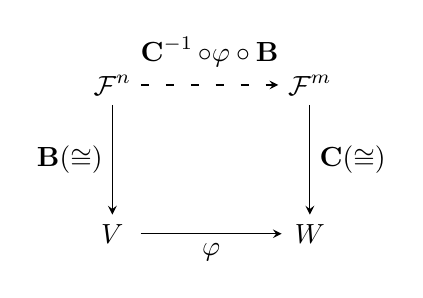
\begin{tikzpicture}
		\matrix (m) [matrix of math nodes,row sep=4em,column sep=5em,minimum width=2em]
		{
			\FF^n & \FF^m \\
			V & W \\};
		\path[-stealth]
		(m-1-1) edge node [left] {$\hv (\cong)$} (m-2-1)
		edge [loosely dashed] node [above=3pt] {$\hvc^{-1} \circ \varphi \circ \hv $} (m-1-2)
		(m-2-1.east|-m-2-2) edge node [below] {$\varphi$}
		node [above] {} (m-2-2)
		(m-1-2) edge node [right] {$\hvc (\cong)$} (m-2-2);
		%edge [dashed,-] (m-2-1);
	\end{tikzpicture}
\end{figure}
This map can only be described based on some choice of bases. The matrix of linear transformation is unique based on the choice of bases.

An important proposition is the following.

\begin{proposition}
	Let \(V\) and \(W\) be finite-dimensional vector spaces over a field \( \F \) and let \(\varphi : V\to W\) be a linear transformation. Let \(r=\rank \varphi\), \(n=\dim V\), \(m=\dim W\). Show that there are bases \(v_1,\dots, v_n\in V\) and \(w_1,\dots, w_m\in W\) such that
	$$\varphi(v_i)=\begin{cases} w_i & \text{ if $i=1,\dots,r$ } \\ 0 & \text{ if $i=r+1,\dots,n$.}\end{cases}$$
\end{proposition}

The story gets a little more complicated if we have two vector spaces of the \textit{same dimension}. Changing the commutative diagram so that $W$ is replaced by $V$ yields that the new matrix is $A = \hv^{-1} \varphi \hv $. This severely restricts the matrix of linear transformation. In particular, consider the following. Let $\hv ' = (v_1' , \dots, v_n')$ be a basis for $\Vdash$. Then the matrix of linear transformation of $\varphi$ and $\hv'$ is $A' = (\hv')^{-1} \varphi \hv'$. Here, note that $A$ and $A'$ are conjugate of one another, ie.
\begin{align*}
A'&=  [(\hv')^{-1} \hv] \varphi [\hv^{-1} \hv]' \\
&= [(\hv')^{-1} \hv] \varphi [(\hv')^{-1} \hv]^{-1}
\end{align*}
Let us generalise this finding.

\begin{proposition}
	\label{sameltunderconjugation}
	Two matrices represent the same linear transformation in different bases \textit{iff} they are conjugates.
\end{proposition}

%Matrix conjugates share some interesting properties; recall from linear algebra over $\R$ that, if $A$ and $B$ are conjugates\footnote{$N(B)$ denotes the null space of vector space $B$.}:
%\begin{itemize}%[noitemsep]
%	\item $\rank B = \rank ABA^{-1}$
%	\item $\dim N(B) = \dim N(A B A^{-1} )$
%	\item $N( ABA^{-1} ) = A \times N(B)$
%	\begin{proof}
%		Let $v \in N(B)$. Then, $Bv = 0$. Then, $ABA^{-1} A v  = A(Bv) = 0$. This proves one inclusion. Another comes from applying definiton of $A \times N(B)$.
%	\end{proof}
%\end{itemize}

To see \propref{sameltunderconjugation} at work, it requires us to understand that two matrices can represent the same linear transformation \textit{but in different coordinate systems}. In particular, we use the following example.

\begin{example}
	Let
	$$ A = \left[\begin{array}{ c c} 2 & 0 \\ 0 & \frac{1}{2} \end{array}\right], \quad B = \left[\begin{array}{ c c}  \frac{1}{2} & 0 \\ 0 & 2 \end{array}\right] $$
	which, obviously, represent the same linear transformation, but one requires you to see the $\R^2$ plane from a different orientation. These matrices are conjugates of one another, ie. if we take
	$$ M = \left[\begin{array}{ c c}  0 & -1 \\ 1 & 0 \end{array}\right]  $$
	then we can verify that $B = MAM^{-1}$ (note that $M$ above is the counterclockwise rotation matrix).
\end{example}

\begin{proposition}
	The general idea is that if we let $A,B,M \in \Ma_{m \times n } (\FF)$, and suppose $M$ is invertible, $B=MAM^{-1}$. Then,
	$$ \left\{ \begin{array}{r c l}
	v & \overset{ A }{\longmapsto } & Av \\
	Mv & \overset{ B }{\longmapsto } & BMv  \\
	& & =  (MAM^{-1}) Mv = MAv \\
	\end{array} \right. $$
\end{proposition}

Some consequences of conjugate matrices follow directly.

\begin{remark}
\begin{itemize}%[noitemsep]
	\item $Av = 0 \iff BMv = MAv = 0$, which implies $\NA (B) = M \times \NA (A)$
	\item (Set of \textit{fixed points}) $Av = v \iff BMv = Mv$, which implies $\fix (B) = M \fix (A)$.
\end{itemize}
\end{remark}

What is interesting is beyond what we can directly observe. In particular, we see that the coordinate system is preserved by \textit{eigenvectors}. 

\begin{definition}
	\textbf{Eigenvectors} are vectors $v \in \FF^n \suchthat Av = \lambda v$ for some $\lambda \in \FF$, where $v \neq 0$.
\end{definition}

\begin{definition}
	\textbf{Eigenvalue} is $\lambda$ given in the previous definition.
\end{definition}

\begin{definition}
	The \textbf{eigenspace} of $\lambda$ is the set
	$$ E_{\lambda} = \left\{ v \in \FF^n \mid Av = \lambda v \right\} $$
\end{definition}

\begin{remark}
	An eigenspace is a vector subspace of a vector space $A$.
\end{remark}

\begin{remark}
	$\NA (A) = E_{0} (A)$, and $\fix (A) = E_{1} (A)$.
\end{remark}

\begin{remark}
	If $B=MAM^{-1}$, $\lambda \in \FF$, then $Av = \lambda v \iff BMv = MA v = M \lambda v = \lambda Mv$. Hence,
	$$ \lambda \in E_{\lambda} (A) \iff M \lambda \in E_{\lambda} (B) $$
	Therefore, we reach the conclusion that $E_{\lambda } (B) = M E_{\lambda} (A)$, $\forall \lambda \in \FF$.
\end{remark}

With these remarks, we can construct the following proposition.

\begin{proposition}
	If $A,B \in \Ma_{n \times n} (\FF)$, and they are conjugates of one another, then eigenvalues of $A$ and $B$ are the same. Furthermore, $\forall \lambda \in \FF$, $\dim (E_{\lambda} (A) ) = \dim (E_{\lambda} (b) ) $.
\end{proposition}

\begin{remark}
	\label{conversefalse1}
	The converse generally does not hold true, \textit{unless we are working over the field fo complex numbers}. Let us see the concept in the following example.
\end{remark}

\begin{example}
	Again, take the rotation matrix
	$$M = \left[\begin{array}{ c c}  0 & -1 \\ 1 & 0 \end{array}\right] $$
	and this has no eigenvalues and eigenvectors over $\R$: note that the characteristic polynomial is
	\begin{align*}
	\det (M - \lambda I) &= \lambda^2 + 1 = 0 \\
	\implies \lambda &= \pm i
	\end{align*}
	Let $\chi_{A}$ denote the characteristic polynomial of matrix $A$. In this case, we say $\chi_{A}=0$ has solutions $x_1 = i$, and $x_2 = -i$.
\end{example}

The following idea is the most profound that we've come across so far. This is provided sans proof in this case, but is germane to this discussion.

\begin{theorem}[Fundamental Theorem of Algebra]
	\label{fundamentalthmofalgebra}
	Let $f(\lambda) $ be a polynomial of the form
	$$ f(\lambda) = a_n \lambda^n + \dots + a_1 \lambda + a_0 $$
	where $n>0$, $a_n \neq 0$, and $\{a_k \}_{k=1}^{n} \in \Com$. Then, $\exists \lambda_0 \in \Com \suchthat f(\lambda_0) =0$.
\end{theorem}

\begin{remark}
	Complex number $\Com$ is not the only field that \thmref{fundamentalthmofalgebra} holds; in general, if we replace $\Com$ with algebraic relations, then we still get the same result.
\end{remark}

\begin{remark}
	\label{consequencesofconjugacy}
	A natural question to ask is \textit{when are two matrices over $\Com$ conjugates of one another}? We note two direct consequences:
	\begin{itemize}
		\item If $A$ and $B$ are conjugates, then the eigenvalues are the same, and $\dim (E_{\lambda} (A) ) =\dim (E_{\lambda} (B) )$.
		\item If $A$ and $B$ are conjugates, then $\chi_A =\chi_B$.
	\end{itemize}
\end{remark}

\begin{remark}
	Similar to \remref{conversefalse1}, we note that \remref{consequencesofconjugacy} contains \textit{only necessary conditions}. In general, they are not sufficient. The following makes the discussion of conjugate matrices a lot clearer.
\end{remark}

\begin{theorem}
	If $A \in \Ma_{n \times n} (\Com)$ and $\chi_A$ has $n$ distinct roots, then the following are equivalent:
	\begin{enumerate}%[noitemsep]
		\item $A$ is diagonalisable
		\item $A$ is conjugate to the diagonal matrix
		\begin{equation}
		\label{eigenvaluediagmatrix}
		\tag{$\triangle$}
		\Lambda = \left[ \begin{array}{c c c c}
		\lambda_1 & & & \\
		 & \lambda_2 & & \\
		 & & \ddots & \\
		 & & & \lambda_n
		\end{array} \right]
		\end{equation}
	\end{enumerate}
\end{theorem}

\begin{proof}
	The proof of this theorem is due to linear algebra over $\R$.
\end{proof}

\begin{remark}
	Therefore, if $A$ and $B$ are such that $\chi_A=\chi_B$, and these characteristic polynomials have distinct roots, then $A$, $B$ are conjugate to \eqref{eigenvaluediagmatrix}.
\end{remark}

\begin{example}
	Take a strictly upper triangular matrix
	$$ D = \left[ \begin{array}{ c c c }
	& 1 & 2 \\
	& & 3\\
	& & 
	\end{array} \right] $$
	where the blank entries are zeros. Then, $\chi_D = \lambda^3 = 0 \implies \lambda_1=\lambda_2=\lambda_3=0$, so the eigenvalues are 0, with multiplicity 3. What is the simplest matrix that is conjugate to $D$? Well, take $E= 3 \times 3$ zero matrix and we're done. However, the zero matrix is only conjugate to itself, ie. let $\mathbf{0}$ denote the $3 \times 3$ zero matrix; then,
	$$ M \mathbf{0} M^{-1} = \mathbf{0} \implies M \in GL_{3} (\Com) $$
\end{example}

Diagonalisation is generally quite difficult to achieve (save for applying singular value decomposition when working over $\R$); we have a close relative to diagonalisation that we will introduce briefly, sans proof, below. It is best motivated by an example.

\begin{example}
	Let $v = \left( \begin{array}{c} -2 \\ 1 \\ 1 \end{array} \right) \in \Com^3$. Furthermore, let $Av = \left( \begin{array}{c} 3 \\ 3 \\ 0 \end{array} \right), A^2 v = \left( \begin{array}{c} 3 \\ 0 \\0  \end{array} \right) , A^3 v = \left( \begin{array}{c} 0 \\ 0 \\ 0 \end{array} \right)  $. We can verify that $Av, A^2 v, A^3 v$ form a basis, and that
	$$ v \overset{A}{\longmapsto} Av \overset{A}{\longmapsto}  A^2 v \overset{A}{\longmapsto}  A^3 v = 0$$
	so the matrix $A$ w.r.t. this basis is
	$$\bordermatrix{  &v &Av &A^2 v \cr
		v& 0 &  0  & 0 \cr
		Av&1  &  0  & 0 \cr
		A^2 v& 0 &  1  & 0 } $$
	This is a very nice result, one we refer to by a proper name.
\end{example}

\begin{theorem}[Jordan Decomposition Theorem]
	\label{Jordan Decomposition Theorem}
	If $A \in \Ma_{n \times n} (\Com)$, then $A$ is conjugate to a matrix of the form
	$$ B = \left[ \begin{array}{c c c c }
	B_1 & & & \\
	& B_2 & & \\	
	&  & \ddots & \\	
	&  & & B_n \\			
	\end{array} \right]$$
	where $B_i$, $\forall i$, is a \textbf{Jordan block}.
\end{theorem}

\begin{definition}
	A \textbf{Jordan block} is of the following form:
	$$ \left[\begin{array}{c} \lambda \end{array}\right] ,\left[\begin{array}{c c} \lambda & \\ 1 & \lambda \end{array}\right], \left[\begin{array}{c c c} \lambda &  & \\ 1 & \lambda &  \\ & 1 & \lambda \end{array}\right], \dots, \left[\begin{array}{c c c c c} \lambda &  & & & \\ 1 & \lambda & & &  \\ & 1 & \lambda & & \\ & & \ddots & \ddots & \\ &  & & 1 & \lambda \end{array}\right] $$
\end{definition}

\begin{remark}
	Every matrix $A \in \Ma_{n \times n} (\Com)$ is conjugate to the form $B$ in \thmref{Jordan Decomposition Theorem}. Take a simple example: \eqref{eigenvaluediagmatrix} matrix. Then, this is diagonalisable iff all Jordan blocks are single blocks, $1 \times 1$ matrix.
\end{remark}

\begin{remark}
	Why is this theorem useful? Well, if we have figured out the number of distinct eigenvalues, and the multiplicities of those eigenvalues, we can figure out the appropriate Jordan block matrix that the matrix of interest is conjugate to.
\end{remark}

\clearpage

\section{Orthogonal Groups}

The idea of this section is fairly simple: we want to study more about matrix groups. So far, we've encountered the following:
\begin{align*}
GL_n (\FF) &= \{\text{ invertible matrix of size } n \times n \} \\
T_n (\FF) &= \{\text{ upper-triangle matrix of size } n \times n \}
\end{align*}
where these matrices admit coefficients from field $\FF$.

\begin{example}
	If we have $v \ in \FF^n$, then we define \textbf{stabilizer of $v$} as
	$$ \stab v = \{ A \in GL_n (\FF) \mid Av = v \} $$
	We can verify that this is a subgroup of $GL_n (\FF)$:
	\begin{itemize}%[noitemsep]
		\item Contains the identity matrix $I_n$
		\item Closed under multiplication: if $A$, $B$ $\in \stab (v)$, then $ABv = Av = v$
 		\item Closed under inverses: if $A \in \stab (v)$, then $Av = v \implies A^{-1} Av = A^{-1} v = v$.
	\end{itemize}
\end{example}

\begin{definition}[Basic vector operations]
	If $\vec{v}, \vec{w} \in \FF^n$, and, WLOG, let
	\begin{align*}
		\vec{v} &= (v_1,v_2,\dots,v_n)\\
		\vec{w} &= (w_1,w_2,\dots,w_n)		
	\end{align*}
	then define
	\begin{itemize}%[noitemsep]
		\item $\langle \vec{v},\vec{w} \rangle = v_1 w_1 + \dots + v_n w_n $
		\item $\norm{\vec{v}} = \sqrt{ \langle \vec{v},\vec{v} \rangle } = \sqrt{v_1^2 + \dots + v_n^2}$
		\item These vectors are \textbf{orthogonal} if $\langle \vec{v},\vec{w} \rangle = 0$
		\item These vectors are \textbf{orthonormal} if $\langle \vec{v},\vec{w} \rangle = 0$, and $\norm{\vec{v}}= \norm{\vec{w}}= 1$.
	\end{itemize}
\end{definition}

\begin{remark}
	A set of vectors $V = \{ \vec{v}_i  \}_{i=1}^{n}$ is orthonormal if, $\forall i,j$,
	$$ \langle \vec{v}_i,\vec{v}_j \rangle = \begin{cases}
	0 & \text{ if } i \neq j \\
	1 & \text{ if } i = j	
	\end{cases}$$
	so the set $V$ has linearly independent vectors, and $V$ is an orthonormal basis.
\end{remark}

\begin{theorem}[From linear algebra over $\R$]
	\label{thm1orthogmatrix}
	If $A \in \Ma_{n \times n} (\R)$, then the following are equivalent:
	\begin{enumerate}%[noitemsep]
		\item $\forall \vec{v} \in \R^n$, $\norm{\vec{v}} = \norm{A \vec{v}}$ ($A$ preserves the length of $\vec{v}$)  
		\item $\forall \vec{v}, \vec{w} \in \R^n$, $ \langle A \vec{v},A \vec{w} \rangle = \langle \vec{v},\vec{w} \rangle	$
		\item $A^T A = I \iff A A^T = I $
		\item Columns of $A$ form an orthonormal basis
		\item Rows of $A$ form an orthonormal basis
	\end{enumerate}
\end{theorem}

\begin{definition}
	Any matrix $B$ satisfying the conditions in \thmref{thm1orthogmatrix} is an orthogonal matrix.
\end{definition}

\begin{properties}
	The following are properties of an orthogonal matrix $A$:
	\begin{enumerate}%[noitemsep]
		\item $ \det (A) = \pm 1$, because
		\begin{align*}
			\det (A^T A) &= \det (I) \\
			\det (A^T) \det (A) &= 1 \\
			[\det (A)]^2 & = 1 \\
			\implies \det (A) &= \pm 1
		\end{align*}
		
		\item $A^{-1}$ is orthogonal: since $A$ is orthogonal, the columns of $A$ are orthonormal, which
		\begin{align*}
		\implies A^{-1} &= A^T \\
		\implies &\text{rows of } A^{-1} \text{ are orthonormal} \\
		\implies & A^{-1} \text{ is an orthogonal matrix}		
		\end{align*}
		
		\item $A$, $B$ orthogonal implies $AB$ is orthogonal matrix, because
		\begin{align*}
		\forall v \in \FF^n, \quad \norm{A(Bv)}  = \norm{Bv} = \norm{v} 
		\end{align*}
		by condition 1 in \thmref{thm1orthogmatrix}. 
	\end{enumerate}
\end{properties}

\begin{definition}
	\label{deforthogonalgroup}
	The set of orthogonal $n \times n$ matrices admitting coefficients in field $\FF$ is denoted $O_n (\FF)$ (the \textbf{orthogonal (matrix) group}). Furthermore, $O_n (\FF) \leq GL_n (\FF)$.
\end{definition}

\begin{definition}
	The \textbf{special orthogonal group} admitting coefficients in field $\FF$, denoted $SO_n (\FF)$, is defined
	$$ SO_n (\FF) = \{ A \in O_n (\FF) \mid \det (A) = 1 \} $$
\end{definition}

We want to first characterise the set of actions we can perform in lower dimensions. We begin with $n=2$, ie. studying $O_2$. In particular, we want to know what transformations preserve the lengths in two dimensions.

\begin{definition}
	A \textbf{rotation} in $\R^2$ is characterised by matrix $R_{\theta}$, where $\theta$ is the angle of rotation.
\end{definition}

\begin{definition}
	The \textbf{rotation matrix} in two dimensions is constructed by choosing the ``canonical'' set of vectors as our basis, ie. take
	$$ e_1 = \left(\begin{array}{c}  1 \\0  \end{array}\right) , \quad e_2 = \left(\begin{array}{c} 0 \\ 1  \end{array}\right) $$
	and coordinates of $R_{\theta}$, under these basis vectors, are
		$$ R(e_1) = \left(\begin{array}{c}  \cos \theta \\ \sin \theta \end{array}\right) , \quad R(e_2) = \left(\begin{array}{c} - \sin \theta \\ \cos \theta  \end{array}\right) $$
	the matrix of linear transformation (rotation) is therefore
		$$ T = \left[\begin{array}{ c c }  \cos \theta &  - \sin \theta \\ \sin \theta  & \cos \theta  \end{array}  \right] $$
\end{definition}

\begin{definition}
	\textbf{Reflection} is a little more difficult to characterise. Specially, we want our choices of \textit{basis vectors/eigenvectors to be orthogonal}---even though we know that, in $\R^2$, as long as we have two non-parallel direction vectors, we have a basis. We can then define two reflections (of basis vectors $\vec{w}_1$ and $\vec{w}_2$) as
	\begin{align*}
	 S_{\theta} w_1 & = w_1 \\
	 S_{\theta} w_2 & = - w_2  
	\end{align*}
	where $S_{\theta}$ is the reflection through line with angle $\theta$ with $x$ axis. Then, we get that these have eigenvalues $1$ and $-1$. In general, we construct
	\begin{align*}
		w_1 \quad &\text{with angle } \theta \\
		w_2 \quad &\text{with angle } \theta + \frac{\pi}{2}
	\end{align*}
\end{definition}

\begin{remark}
	Such reflection matrix $S_{\theta}$ can also be characterised w.r.t. conjugation. To be clear, take the rotation matrix $R_\theta$, and define $S'_{\theta}$ as
	\begin{align*}
		S'_{\theta} &= \left[ \begin{array}{ c c }  \cos \theta &  - \sin \theta \\ \sin \theta  & \cos \theta  \end{array}\right] \left[ \begin{array}{ c c }  1 &  0 \\ 0  & 1  \end{array}\right]  \left[ \begin{array}{ c c }  \cos \theta &  - \sin \theta \\ \sin \theta  & \cos \theta  \end{array}\right]^{-1}  \\
		&= \left[ \begin{array}{ c c }  \cos 2 \theta &  \sin 2 \theta \\ \sin 2 \theta  & - \cos 2 \theta  \end{array}\right]  \coloneqq \bar{A}
	\end{align*}
	and we notice that $\bar{A}= \bar{A}^{-1}$, so this is indeed a reflection matrix.
\end{remark}

\begin{theorem}
	\label{matrixtheoremO2}
	$M \in O_2$ is either
	\begin{itemize}%[noitemsep]
		\item rotation matrix ($\det M =1$); or,
		\item reflection matrix ($\det M =-1$).
	\end{itemize} 
\end{theorem}

\begin{proof}
	If $M $ is orthogonal, then it has orthonormal columns. Then, $\exists \theta \in [0,2\pi] \suchthat $
	$$ M = \left[\begin{array}{c c} \cos \theta & x \\ \sin \theta & y \end{array} \right]$$
	where we want $\norm{ (x,y) } =1$, and $\langle (x,y), (\cos \theta, \sin \theta) \rangle = 0$. Hence, we want
	\begin{align*}
	x \cos \theta + y \sin \theta &= 0 \\
	\implies (x,y ) & = t (\sin \theta, - \cos \theta ) \\
	\implies \langle (x,y) \rangle &= \abs{t} \\
	\implies t &= \pm 1
	\end{align*}
	hence, $(x,y) = \pm (\sin \theta, -\cos \theta)$. Then we get either of the following:
	$$ M = 
	\begin{cases}
	\left[\begin{array}{c c} \cos \theta & \sin \theta \\ \sin \theta & -\cos \theta \end{array}\right] & = S_{\frac{\pi}{2}} \\
 	\left[\begin{array}{c c} \cos \theta & -\sin \theta \\ \sin \theta & \cos \theta \end{array}\right]  &  = R_{\theta}
	\end{cases}
	 $$
\end{proof}

\begin{corollary}
	\begin{itemize}%[noitemsep]
		\item Composition of rotations is rotation
		\item Composition of reflections is rotation.
		\item Composition of rotation and reflection is a reflection.
	\end{itemize}

	This is easily deduced by multiplying two matrices and looking at their determinants.
\end{corollary}

\clearpage

\section{Isometries and Isometry Group}

From \defnref{deforthogonalgroup}, we see that any orthogonal matrix $A \in \Ma (\R)$ satisfies the property that $\forall v \in \R^n$, $\norm{Av} = \norm{v} $. 

\begin{definition}
	An \textbf{isometry} of $\R^n$ is a map
	$$\varphi : \R^n \mapsto \R$$
	$\suchthat \forall v,w \in \R^n$, $\norm{v-w} = \norm{\varphi(w) - \varphi(w) }  $.
\end{definition}

\begin{remark}
	A map that preserves lengths automatically preserves distances.
\end{remark}

\begin{remark}
	A few objects we've studied are isometries:
	\begin{itemize}%[noitemsep]
		\item Orthogonal linear transformations are isometries:
		\begin{align*}
			\forall v,w \in \R^n, &\quad \forall M \in O_n \\
			\norm{Mv - Mw} &= \norm{ M(v-w)}   \\
			&= \norm{v-w} 
		\end{align*}
		
		\item Translations are isometries: let $a\in \R$; let
		$$		 \fullfunction{t_a}{\R^n}{\R}{x}{x+a} $$
		then this
		\begin{align*}
		\implies t_a(v)-t_a (w) &= \norm{ v+a - (w+a) }  \\
		&= \norm{v-w} 
		\end{align*}
		
		\item Compositions of isometries are isometries: let $f,g$ be isometries, defined
		$$f,g : \R^n \mapsto \R$$
		then it must be the case, for $f\circ g$, that $\forall v,w\in \R^n$,
		\begin{align*}
			\norm{ (f\circ g)(v) - (f\circ g)(w) } &= \norm{ f(g(v)) - f(g(w)) }  \\
			&= \norm{g(v) - g(w) } = \norm{v-w} 
		\end{align*}
	\end{itemize}
\end{remark}

We state the following in full; the proof is in Artin, which is omitted because it is less than instructive.

\begin{theorem}
	\label{thmisometriesofRn}
	Every isometry of $\R^n$ is a composition of an orthogonal matrix and a translation. In particular, if $f: \R^n \mapsto \R$ is an isometry, then $\exists! a\in \R^n$, $M \in O_n \suchthat f = t_a \circ M$.
\end{theorem}

There are a few direct consequences of \thmref{thmisometriesofRn}; we state a couple of them.

\begin{corollary}
	The set of isometries in $\R^n$ forms a group; let us denote it $\isom_n$, we law of composition as the composition of maps.
\end{corollary}

\begin{proof}
	Check the usual conditions:
	\begin{enumerate}%[noitemsep]
		\item Closure under group operation
		\item Identity element: compose identity matrix and identity function (translation)
		\item Inverse: if $f = t_a \circ M$, for some $a \in \R^n$, $M \in O_n$, then
		\begin{align*}
		f^{-1} &= (t_a \circ M)^{-1} \\
		&= M^{-1} \circ t_{-a}
		\end{align*}
		and we know such inverse matrix exists because the definition of orthogonal matrix says that such $M$ satisfies $M^T M = I$.
	\end{enumerate}
\end{proof}

\begin{properties}[of the isometry group]
	\begin{itemize}%[noitemsep]
		\item If $M \in O_n$, $a \in \R^n$, then
		\begin{align*}
			M \circ t_a (x) &= M(x+a) = Mx+Ma \\
			&= (t_{Ma} \circ M) (x) \\
			\implies M \circ t_a &= t_{Ma} \circ M
		\end{align*}
		
		\item $\forall a,b \in \R^n$, $t_a t_b = t_{a+b}$

		\item If $a \in \R^n$, $f \in \isom_n$ (in particular, $f = t_b \circ M$), then
		\begin{align*}
			f \circ t_a  \circ f^{-1} &= t_b \circ M \circ t_a \circ M^{-1} \circ t_b^{-1} \\
			&= t_b  \circ (t_{Ma} \circ M) \circ M^{-1} \circ t_b^{-1} \\
			&= t_b  \circ t_{Ma} \circ (M \circ M^{-1}) \circ t_b^{-1} 	\\
			&= t_b  \circ t_{Ma} \circ t_b^{-1} = t_{Ma}
		\end{align*}
		which is just a translation; hence, conjugation of translation by isometry is still a translation.

		\item Denote the group of translation $T$. $T \lhd \isom_n$.
	\end{itemize}
\end{properties}

\begin{remark}
	Of course, we can prove that $T \lhd \isom_n$ if we construct a homomorphism $\pi$, with the property $\ker \pi = T$. Let us preserve the linear part of the translation---the derivative of the translation, ie.
	$$\fullfunction{\pi}{\isom_n}{O_n}{t_a \circ M}{M}$$
	check that this is indeed a homomorphism:
	\begin{align*}
		\pi (t_a M M' t_b) &= \pi ( t_a t_{Mb} M t_b ) \\
		&= \pi ( t_{a+Mb} M M' ) = M M'
	\end{align*}
	with $\ker \pi = \{\text{translations} \}$.
\end{remark}

\begin{definition}
	Let $f \in \isom_n$. Then, we say
	\begin{enumerate}%[noitemsep]
		\item $f$ is \textbf{orientation-preserving} if $\det (\pi (f) ) = 1$; and
		\item $f$ is \textbf{orientation-reversing} if $\det (\pi (f) ) = -1$,	
	\end{enumerate}	
	where
	$$	\fullfunction{\pi}{\isom_n}{O_n}{t_a \circ M}{M}$$
	is the derivative map we've defined above.
\end{definition}

Again, we study only isometries of lower dimension spaces. It is particularly interesting to study $\isom_2$. We have a nice classification theorem as follows.

\begin{theorem}
	\label{isom2categories}
	Every isometry of $\R^2$ falls into either one of the four categories:
	\begin{enumerate}%[noitemsep]
		\item \textbf{Translation}
		\item \textbf{Rotation} around some point in the plane
		\item \textbf{Reflection} through some line $\ell$
		\item \textbf{Glide reflection}: reflection through $\ell$, then translation parallel to $\ell$
	\end{enumerate}
\end{theorem}

\begin{proof}
	In order to prove \thmref{isom2categories}, we need to prove the following lemmas; we prove them one by one.
	
	\begin{lemma}
		\label{lemmaoptransrot}
		\textit{All} orientation-preserving isometries are either translations or rotations. 
	\end{lemma}

	\begin{proof}[Proof of \lemref{lemmaoptransrot}]
		The idea is as follows. Let $f: \R^2 \mapsto \R^2$ be a rotation of a point $x$ by angle $\theta$, around some point $P$. Let us denote distances: $(x-p)$ for the first coordinate, and $f(x)-p$ for the second coordinate. But, with some calculations, we can show that
		\begin{align*}
		f(x) - p &= R_{\theta} (x-p) \\
		\implies f(x)&= R_{\theta} (x-p) + p \\
		&= t_p \circ R_{\theta} \circ t_{-p} 
		\end{align*}
		Then, let $f = t_a \circ M_2$, where $a \in \R^2$, $M \in O_2$. Then, $\det M =1$, and $M = R_{\theta}$ for some $\theta \in [0,2\pi)$. Then, there are two subcases:
		\begin{enumerate}%[noitemsep]
			\item $\theta =0 \implies M=R_0 = id$. Hence, $f$ is a translation.
			\item $\theta \neq 0 \implies f$ is a rotation. How do we see this? We need to first solve for a fixed point $p$, ie. the point of rotation. Hence,
			\begin{align*}
			t_a \circ M &= p \\
			\implies t_a \circ R_{\theta} p &= p \\
			\implies a &= (I - R_{\theta}) p
			\end{align*}
			and $(I- R_\theta)$ needs to be invertible in order for us to solve $p$; a direct computation yields
			\begin{align*}
			\det (I- R_\theta)&= \det \left[ \begin{array}{c c} 1 - \cos \theta & -\sin \theta \\ \sin \theta & 1 - \cos \theta \end{array} \right] \\
			&= 1 - 2\cos \theta + \cos^2 \theta + \sin^2 \theta \\
			&= 2 - 2 \cos \theta \neq 0
			\end{align*}
			since $\theta \neq 0, 2\pi, \dots, n\pi$, where $n \in \Z 2$. Hence, $\exists! p \in \R^2 \suchthat f(p)=p$. Hence, $f$ is a rotation by $\theta$ around some point $p$. Lastly, we just want to show that $f$ is well-defined:
			\begin{align*}
			t_p \circ R_{\theta} \circ t_{-p} &=t_p \circ t_{R_\theta (-p)} \circ R_\theta \\
			&=  t_{ p (I - R_\theta) } \circ R_\theta \\
			&=   t_{ a} \circ R_\theta 			
			\end{align*}
			as desired.
		\end{enumerate}
	\end{proof}
	
	\begin{lemma}
		\label{lemmaorrefgf}
		Every orientation-reversing $f \in \isom_2$ is either a reflection or a glide-reflection.
	\end{lemma}

	\begin{proof}[Proof of \lemref{lemmaorrefgf}]
		The idea is fairly simple. Assume, WLOG, $f=t_a \circ S_\ell$, where $S_\ell$ is a reflection through line $\ell$. Define $u$, $v$ by choosing a particular coordinate, and make sure such vector passes through the origin. Then, change the coordinates such that line $\ell$ is the $u$-axis. Then, we can say that
		\begin{align*}
		S_{\ell} (u,v) &= (u,-v) \\
		\implies t_a \circ S_{\ell} (u,v) &= (u,-v) + (a_1, a_0) \\
		&= (u+ a_1,a_0 -v)
		\end{align*}
		and this is a glide reflection through $\ell' = \left\{ v = \frac{a_2}{2} \right\}$, and translation by $(a_1,0)$. Hence, we can (algebraically) say that
		\begin{align*}
			S_{\ell' } (u,v) &= (u,a_2-v) \\
			\implies t_{(a,0)} \circ S_{\ell'} &= (u,a_2-v) + (a_1,0) \\
			&= (u+a_1,a_2 - v)
		\end{align*}
		which demonstrates the fact that any such $f$ is well-defined.
		
		Now, if $a_1=0$, then we have a translation; if $a_1 \neq 0$, we have a glide reflection.
	\end{proof}
	
	Combining both \lemref{lemmaoptransrot} and \lemref{lemmaorrefgf} proves the theorem we want to prove.
\end{proof}

A particularly powerful way to study groups of lower dimensions, such as $O_2$, is to classify the \textit{finite subgroups} of such groups. Let us consider classifying finite subgroups of $O_2$---which can be understood as symmetry groups of some geometric figures. We are ultimately interested in proving the following theorem.

\begin{theorem}
	\label{thmclassificationfsgrpO2}
	Let $G$ be a finite subgroup of $O_2$. Then, $\exists n>0 \suchthat $ either 
	\begin{enumerate}%[noitemsep]
		\item $G$ is a cyclic group of order $n$, generated by rotation $R_{\frac{2\pi}{n}}$; or,
		\item $G= D_n$, the dihedral group of order $2n$.
	\end{enumerate}
\end{theorem}

We cannot begin to prove this theorem, unless we have more structures to work with. In particular, we want to define a dihedral group, and describe a couple of properties of such group.

\begin{definition}
	\textbf{Dihedral group} of order $n$, denoted $D_n$, is a group generated by 2 elements:
	\begin{align*}
	R_{\frac{2\pi}{n}} &\coloneqq R\\
	S_{\ell} &\coloneqq S
	\end{align*}
\end{definition}

\begin{example}
	Let us examine $D_3$. This is the group of symmetries of an equilateral triangle. Such triangle has three lines of symmetry---each from a vertex to the midpoint of its opposite side. This is indeed a group: we can define all the elements in this group from the collection of symmetries on equilateral triangles,
	$$ \left\{ id, R_{\frac{2\pi}{3}} , R_{\frac{4\pi}{3}} , S_{\ell_1} , S_{\ell_2} , S_{\ell_3} \right\} $$
	in particular, we let $R= R_{\frac{2\pi}{3}}$, $R^2 = R_{\frac{4\pi}{3}} $, and $S = S_{\ell_1}$ in the computations below. Then, we can see that
	\begin{align*}
	S \circ R &= \left\{\begin{array}{c c c}
	B & \longmapsto & C \\
	A & \longmapsto & A \\
	C & \longmapsto & B
	\end{array} \right.= S_{\ell_2} \\
	R \circ S &= \left\{\begin{array}{c c c}
	B & \longmapsto & A \\
	A & \longmapsto & B \\
	C & \longmapsto & C
	\end{array} \right.	 = S_{\ell_3}
	\end{align*}
	so compositions of reflection with rotation (in any order) gives reflection. Hence, $D_3$ is the set
	$$ \left\{ id, R, R^2, S, SR, SR^2 \right\} $$
	equipped with composition.
\end{example}

\begin{remark}
	We claim that $D_3 \cong S_3$. Recall that we can always define $S_3$ using two generators: $x=(123)$ and $y=(12)$, for example. And, we can then define $SR^{-1} = RS$, resulting in a one-to-one correspondence between the elements generated by these elements.
	
	Another way of seeing the existence of this isomorphism is to construct a homomorphism: namely,
	$$\fullfunction{\varphi}{D_3}{S_3}{f}{\text{permutations of vertices induced by } f}$$
	and map all elements in $D_3$ to exactly one element in $S_3$.
\end{remark}

\begin{remark}
	The size of $D_n$ is generally much smaller than the size of $S_n$; in particular, $\abs{D_n} = 2n$ while $\abs{S_n}=n!$.
\end{remark}

\begin{proposition}
	The generators of $D_n$ satisfy the following relations:
	\begin{itemize}%[noitemsep]
		\item $R^n = id$
		\item $S^2 = id$
		\item $RS = SR^{-1}$
	\end{itemize}
	and $\abs{D_n}=2n$, while the set of the group $D_n$ is
	\begin{equation}
	\label{Dnelements}
	\left\{ \underbrace{id, R, R^2, \dots, R^{n-1}}_{n \text{ rotations}} , \underbrace{S, SR, SR^2, \dots, SR^{n-1}}_{n \text{ reflections}} \right\}
	\end{equation}
\end{proposition}

\begin{proof}
	The idea is to prove that the elements in this set are distinct, and that there are exactly $2n$ elements.
	
	For the first part, we know that rotations and reflections are distinct, hence $R^{i} \neq SR^{j}$, $\forall i,j$.
	
	For the second part, it suffices to prove that elements in \eqref{Dnelements} are closed under multiplication, and have inverses that are in the group. It follows that it suffices to prove closure by multiplication by the two generators of $D_n$,
	\begin{itemize}%[noitemsep]
		\item \uline{Multiplication by $R$}: we have that
		\begin{align*}
			R \cdot R^{j} &= R^{j+1} \in D_n \\
			SR^{i} \cdot R &= S \cdot R^{i+1} \in D_n \\
			R \cdot SR^{i} &= SR^{-1} R^{i} = SR^{i-1} \in D_n
		\end{align*}
		
		\item \uline{Multiplication by $S$}: similarly,
		\begin{align*}
			S \cdot R^{j} & \in D_n \\
			R^{i} S \cdot R &= S \cdot R^{-i} \in D_n \\
			SR^{i} \cdot S &= \underbrace{SS}_{=S^2 = id} R^{-i} = R^{-i} \in D_n
		\end{align*}
	\end{itemize}
	and that inverses are closed:
	\begin{align*}
		(R^i)^{-1} &= R^{-i}
	\end{align*}
	which is defined because $R^{-i}$ would just be a backward/reverse rotation.
\end{proof}

Before we can prove the finite subgroups classification of $O_2$, we need to define one more piece of convention.

\begin{definition}
	A subgroup $\Gamma \leq \R$ is \textbf{discrete} if $\exists \varepsilon>0 \suchthat \forall x \in \Gamma$, either $\abs{x} > \varepsilon$, or $x=0$.
\end{definition}

\begin{example}
	$\Z \leq \R$ is a discrete subgroup. In particular, recall that subgroups of $\Z^+$ is either trivial or of the form $\Z a$, for some least positive integer $a>0$. $\Z a$ is also a discrete subgroup of $\R$.
\end{example}

\begin{example}
	$\Q \leq \R$ is \textit{not} a discrete subgroup, because $\Q$ is dense in $\R$.
\end{example}

We want to prove a quick lemma, as follows.

\begin{lemma}
	\label{lemdiscreteZa}
	Let $\Gamma \leq \R$ be a discrete, non-trivial subgroup. Then, $\exists \alpha >0 \suchthat \Gamma = \Z \alpha$.
\end{lemma}

\begin{proof}
	The proof follows largely by definition. In particular, we need to prove in two steps:
	\begin{enumerate}%[noitemsep]
		\item That $\Gamma$ has a least positive element,
		\item That $\Gamma$ is generated by some $a>0$.
	\end{enumerate}

	The first step is nontrivial because if we define $\left\{x_n\right\} \subset \Q$, where $x_n = \frac{1}{n}$, then we have the case that, $\forall n \in \N$,
	$$x_n = \frac{1}{n} > \frac{1}{n+1} = x_{n+1}  $$
	But we can always define something as follows: $\forall a,b \in \Gamma$, $a-b \in \Gamma$, so by definition of discrete subgroup, $a-b=0$ or $\abs{a-b} > \varepsilon$, for some $\varepsilon >0$. Hence, two consequences can happen:
	\begin{enumerate}%[noitemsep]
		\item $a-b=0\implies a=b$
		\item $b-\varepsilon < a < b+\varepsilon$
	\end{enumerate}
	If we're in the first case, we're done. If we're in the second case, then we can always say that any interval of length $\varepsilon$ contains at most one element of $\Gamma$. In other words, $\exists c \suchthat c\in \Gamma$, and if $c>0 \implies$ we're done; $c<0 \implies$ pick $-c$ to do the trick.
	
	Finally, pick $(0,c]$ as our interval, and cut it into finitely many intervals of length $\varepsilon$. Take $[a,b]$ as teh smallest interval among those intervals (where $a$, $b$ are the least possible values in the intervals we've cleaved).
	
	The second step is to prove that $G = \Z a$, where $a$ is the least positive element of $G$. One inclusion is obvious: $\Z a \subset G$, because $a \in G$. Hence, $\langle a \rangle = \Z a \subset G$. The other inclusion comes from a little less obviously: take $g \in G$; then $\exists N \in \N \suchthat g = na$, which implies $n \leq \frac{g}{a} < n+1$. Hence, multiplying through the inequalities through by $a$
	$$\begin{array}{c c c c c c}
	& an &\leq & g & < & (n+1)a \\
	\implies & 	0 &\leq & g-na & < & a
	\end{array}$$
	but $a$ can be arbitrarily small, hence $g-na=0 \implies g=na$. Hence, $G \subset \Z a $.
	
	Another way to prove second step is as follows: again, one inclusion is obvious---$\Z a \subset G$, because $a \in G$. For the other inclusion, let $g \in G$, and $g = ra $ where $r\in \R$. We write $r = m + r'$, where $m \in \Z$ and $0 \leq r' <1$. Since $G$ is a group, $g' = g - ma \in G$ and $g' = r' a$. Since $0 \leq g' < a$, and $a$ is the least positive integer in $G$, $g' = 0 \implies g- ma= 0 \implies g= ma$. Hence, $G \subset \Z a$.
\end{proof}

Now we're ready to prove \thmref{thmclassificationfsgrpO2}.

\begin{proof}[Proof of \thmref{thmclassificationfsgrpO2}]
	There are two different cases we must consider.
	\begin{enumerate}%[noitemsep]
		\item \uline{$G$ contains rotations only}. Claim: $G \cong C_n$ for some $n$. Consider the set
		$$ A = \left\{ \theta \in \R \mid R_{\theta} \in G \right\} $$
		which is a subgroup of $\R^+$. This contains $R_{2\pi} = R_0 = id$. This is a discrete subgroup because $A$ contains finitely many numbers between $0 $ and $2\pi$. Hence, by \lemref{lemdiscreteZa}, $A = \Z a$, where $a>0$. We know $2\pi$ is in the set; hence,
		\begin{align*}
		2 \pi&= na \\
		\implies a &= \frac{2\pi}{n}
		\end{align*}
		hence
		$$ G = \left\{ R_{\frac{2\pi}{n}}, R_{2 \times \frac{2\pi}{n}}, \dots, R_{ (n-1) \times \frac{2\pi}{n}
		 }  \right\} = \left\langle R_{\frac{2\pi}{n}} \right\rangle \implies G \cong \left\langle R_{\frac{2\pi}{n}} \right\rangle$$
		
		\item \uline{$G$ contains rotations and a reflection}. Let $S$ be a reflection through a line $\ell$. Choose coordinates so that $\ell$ is the $x$-axis. Let
		$$H= \left\{ \text{rotations in } G \right\} = SO_2 \cap G$$
		and $H$ is finite as a subset of $G$, which is a finite group. Hence, by case 1, $\exists n>0 \suchthat H= C_n = \left\langle R_{\frac{2\pi}{n}} \right\rangle$. Hence
		$$ G \supset \left\{ id, R_{\frac{2\pi}{n}}, R_{2 \times \frac{2\pi}{n}}, \dots, R_{ (n-1) \times \frac{2\pi}{n}}, S, R_{\frac{2\pi}{n}} S, R_{2 \times \frac{2\pi}{n}} S , \dots, R_{ (n-1) \times \frac{2\pi}{n}} S \right\} = D_n$$
		The other inclusion is more difficult to show. Suppose $M \in G$. If $M$ is a rotation, then $M \in H  \subset D_n$; if $M$ is a reflection, then $MS $ is a rotation$\implies MS = R_{\frac{2\pi}{n}k}$ for some $k \implies M =R_{\frac{2\pi}{n}k} S^{-1} \in D_n$. Hence, $G \cong D_n$.
	\end{enumerate}
\end{proof}

A much more profound question is to characterise the finite subgroups of $\isom_2$. We define
$$ \isom_2 = \condset{ x \mapsto Mx + a }{ M \in O_2}{,}{ a\in \R^2} $$
and we can see that finite subgroups of $\isom_2$ contains no translations or glide-reflections. This is simply because finite subgroups have elements of finite order.

\begin{theorem}
	\label{thmclassificationisom2}
	A finite subgroup of $\isom_2$ is isomorphic to $C_n$ or $D_n$ for some $n \in \N$.
\end{theorem}

To prove \thmref{thmclassificationisom2}, we need the following lemma.

\begin{lemma}
	\label{lemfixedpointp}
	If $G \subset \isom_2$ is a finite subgroup, then it has a fixed point $p$. In other words, $\exists p \in \R^2 \suchthat g(p)=p$, $\forall g\in G$. 
\end{lemma}

We need to define the following object:

\begin{definition}
	Let $v \in \R^2$. The \textbf{orbit} of $v$ is the set
	$$ Gv = \condset{ g(v) \in \R^2}{ g \in G}{}{} $$
	where $Gv $ is symmetric in $G$.
\end{definition}

\begin{proof}[Proof of \lemref{lemfixedpointp}]
	Let $f \in G$. Then,
	\begin{align*}
	f (Gv) &= \condset{ f(g(v))}{ g \in G}{,}{ v\in R^2} \\
	&= \condset{ (f \circ g)(v) }{ g \in G}{,}{ v\in R^2} \\
	&\subset Gv
	\end{align*}
	Similarly, we know
	\begin{align*}
	f^{-1} (Gv) &\subset Gv \\
	\implies Gv &\subset f(Gv)
	\end{align*}
	therefore, $f(Gv)=Gv$. We conclude that orbit is preserved by an isometry.
\end{proof}

\begin{proof}[Proof of \thmref{thmclassificationisom2}]
	We define the \textit{centroid} as the average of the $Gv$, where, since $G$ is finite, we can write
	$$Gv = \left\{ s_1,\dots,s_n \right\}$$
	and the centroid $c$ can therefore be expressed as
	$$ c= \frac{1}{n} \left( s_1 + \dots + s_n \right) $$
	We claim that $\forall g \in G$, $g(c) =c$. Let $g \in G$. Then, $\exists M \in O_2, v\in \R^2 \suchthat \forall x \in \R^2, \: g(x)=Mx +v$. Then,
	\begin{align*}
		g(c) &= Mc + v \\
		&= M \left( \frac{1}{n} \left( s_1 + \dots + s_n \right) \right) + v \\
		&= \frac{1}{n} M S_1 + \frac{1}{n} M S_2 + \dots + \frac{1}{n} M S_n + v \\
		&= \frac{1}{n} (M S_1 + v) + \frac{1}{n} (M S_2 + v) + \dots + \frac{1}{n} (M S_n + v) \\
		&= \frac{1}{n} (g(s_1) + \dots + g(s_n) ) \\
		&= \frac{1}{n} \left( s_1 + \dots + s_n \right)  =c
	\end{align*}
	where the penultimate equality sign in the last line follows from the fact that $\forall g \in G, g(Gv) = Gv$. Since $c$ is a fixed point, ie. $g(c)=c$ for all $g \in G$, rotation about point $c$ \textit{and} reflection about a line passing through $c$ with angle $\theta$ would be a decent coordinate system to use.
	
	To that end, let $c$ be the origin of the coordinate system, ie. $c=0$. Hence, $g(0)=0$. Then, $G \subset O_2$. And, since $G$ is finite, use \thmref{thmclassificationfsgrpO2} to say that $G$ is either $C_n$ or $D_n$. Hence, any finite subgroup of $\isom_2$ is either $C_n$ or $D_n$, as desired.
\end{proof}

Now, we know it is possible to characterise all finite subgroups of $\isom_2$. Let us try to construct a characterisation of \textit{infinite subgroups of $\isom_2$}. In particular, let us characterise the possible groups of symmetry of a figure in the plane. If I have a rectangular brick tiling, it is possible to define translations, rotations about some point(s), and reflections/glide-reflections if we want; \textit{but} it is not always the case that, if we take a subgroup $G$, we can construct a figure that is symmetric under $G$. If I take a subgroup $G$ generated by two translations and a reflection about a line $\ell$ passing through the origin, with angle $\theta$, then I have exactly
$$G = \left\langle t_a , t_b , s_\ell \right\rangle  $$
where $a,b \in \R^2$, and $s_\ell$ is a reflection about the line $\ell$; the claim is elements in this group is symmetric under $G$. We know this because everything plays out ``nicely'': translations are easy to manipulate, and reflections always produce one corresponding image. But some rather un-nice sets are the following: take
\begin{align*}
	H &=  \cyclic{R_1}  \\
	J &= \condset{ \left(x,y\right)}{x,y}{ \in }{ \Q} 
\end{align*}
where we have an infinite amount of translations in the case of $J$, and an infinite amount of rotations in the case of $H$. There is no way to get back to the identity element $R_0$ if we have a group generated by rotations of 1 radian (as no multiple of $\pi$ is ever an integer). Hence, we need to define the notion of \textit{discreteness of subgroups of $\isom_2$} to make sense of this dichotomy.

\begin{definition}
	A \textbf{discrete subgroup $G$ of $\isom_2$} is where $\exists \varepsilon>0 \suchthat $
	\begin{enumerate}%[noitemsep]
		\item $G$ contains no translations $\vec{a} $ with $\norm{\vec{a}} < \varepsilon$, except the identity element;
		\item $G$ contains no rotations of angle $\theta$ with $\theta < \varepsilon$, except the identity element.
	\end{enumerate}
\end{definition}

Now, a fair amount of work goes into characterising all discrete subgroups of isometry group $\isom_2$; there are two dozens of those subgroups. We will characterise two of them, and explain the connection between them.

\begin{obs}
	From here on, let $G \leq \isom_2$ be a discrete subgroup. Then, we can describe $G$ using
	\begin{itemize}%[noitemsep]
		\item translation subgroups (subgroup consisting only of translations);
		\item point group (subgroup of $O_2$ consisting of linear parts of elements of $G$).
	\end{itemize}
\end{obs}

\begin{description}
	\item[Translation Subgroup] Let $T \subset \isom_2$ where $T = \left\{ \text{translations} \right\} = \left\{ t_a \mid a \in \R^2 \right\}$. Define \textbf{lattice} $L = T \cap G = \left\{ \text{set of translations in } G \right\}$. Hence, we know $L \cong (\R^2,+)$. A particularly powerful theorem can therefore be stated as follows:
	
	\begin{theorem}
		\label{thmclassificationlattice}
		The translation subgroup $L = T \cap G$ is a discrete subgroup of $T \cong (\R^2,+)$. There are only three possible types of $L$:
		\begin{enumerate}%[noitemsep]
			\item $L = \left\langle t_a ,t_b \right\rangle$
			\item $L = \left\langle t_a \right\rangle$
			\item $L = \left\{ e \right\}$			
		\end{enumerate}
		where $a,b \in \R^2$.
	\end{theorem}
	
	\begin{remark}
		The first part of \thmref{thmclassificationlattice} is extremely simple: $L$ is discrete as a subgroup of a discrete subgroup. It is much harder to prove that these are the only cases of subgroups of $T$.
	\end{remark}
	
	\begin{proof}[Proof of \thmref{thmclassificationlattice}]
		\textit{(Developing)}
	\end{proof}

	\item[Point Group] Recall that every element $a\in \isom_2$ is a composition of $M \in O_2$ and translation $a \in \R^2$. Then, it is the case that we can define such $f : \R^2 \mapsto \isom_2 $ as $f(x) = Mx + a$. Again, we can preserve the linear part of this map, ie. define
	$$\fullfunction{\pi}{\isom_2}{O_2}{Mx + a}{M}$$
	where $\pi \left( t_a \circ M \right) = M$. Then, we can define the following:
	
	\begin{definition}
		The \textbf{point group} $\overline{ G}$ of $G$ is defined $\overline{ G} = \pi (G)$.
	\end{definition}
	
	\begin{lemma}
		\label{lempgisdiscretefinite}
		With $G$, as given, $\overline{ G}$ is discrete and finite.
	\end{lemma}

	\begin{idea}
		If $\overline{G}$ contains no small rotations, then it has elements of finite order. Hence, \lemref{lempgisdiscretefinite} makes sense.
	\end{idea}
\end{description}

With these in mind, we want to now develop some connections between translation subgroups and point groups. We continue to denote $G$ as a discrete subgroup of $\isom_2$, and $L $ as the lattice of $G$ as defined above. We make a couple of remarks below.

\begin{remark}
	\label{rmklatticeker}
	$L \lhd G$. In particular, with $\pi$ as above, we see that $L=\ker \pi$.
\end{remark} 

\begin{proof}[Proof of \remref{rmklatticeker}]
	By definition, $\ker \pi = \left\{ f \in L \suchthat \pi (f) = e_{G} \right\}$, and $e_G = I_2$. Hence, any $f \in L$ in the form $I_2 x + a$ is in the kernel of $\pi$. This is precisely the set of translations in $G$, ie. $L$.
\end{proof}

\begin{remark}
	Restrict $\pi$ to $G$. Then, we see that
	$$ \pi|_{G} : G \mapsto \overline{ G} $$
	meaning we have a surjective homomorphism. By First Isomorphism Theorem, we can then write
	$$ \im \pi \cong G / \ker \pi \implies \overline{ G} \cong G / L $$
\end{remark}

\begin{remark}
	\label{obstilingexample}
	Take the tiling diagram in Artin. Observe that translations always work: take two linearly independent vectors, ie. $(0,2)$ and $(1,1)$, to generate the set of translations. Suppose rotation around the centres of these squares, in multiples of $\pi/2$ radians, are the only viable actions. Suppose further that there are reflections about some line $\ell$ passing through the centre of the squares. Then, we can define the point group
	$$ \overline{ G} =\left\{ id, R_{\frac{\pi}{2}} , R_{{\pi}} ,R_{\frac{3\pi}{2}}, S_0, S_{\frac{\pi}{4}}, S_{\frac{\pi}{2}} , S_{\frac{3\pi}{4}} \right\} \cong D_4 $$
\end{remark}

\begin{remark}
	As in \remref{obstilingexample}, and by \thmref{thmclassificationisom2}, we have that $\overline{G} \cong C_n$ or $\overline{G} \cong D_n$. In this case, since we have reflections, it must be the case that $\overline{G} \cong D_n$.
\end{remark}

\begin{remark}
	Obviously, we can denote each element in $\overline{ G}$ using $f_i$, where $i=1,2,\dots,8$, and conclude that, by the quotient group definition of $\overline{ G}$,
	$$ [G:L] = \abs{G/L} = 8 $$
	and, for any $M \in \overline{ G}$, $\pi^{-1} (M)$ is a coset of $L$, and each $f_i$ is in a different coset $L f_i$. Hence,
	$$ G = L f_1 \cup L f_2 \cup \dots \cup L f_8 $$
\end{remark}

With these remarks, we can get at a fairly beautiful lemma, as follows.

\begin{lemma}
	\label{lempgassymmetryofts}
	The point group is a symmetry group of the translation subgroup, ie. $\forall a\in L, f\in G$, $\pi (f) a \in L$, using $\pi$ as defined earlier.
\end{lemma}

\begin{obs}
	If we have a plane of squares of 1 unit lengths, then the set of translations is exactly
	\begin{align*}
	L =\condset{ (x,y)}{ x,y }{\in}{ \Z} = \Z^2
	\end{align*}
	which admits reflections and rotations about some centres, hence $\overline{ G} \cong D_4$, as before. If we have have a plane of rectangles, of size 2 units by 1 unit, then we have
	$$ L = \cyclic{ (2,0) , (0,1)} \implies \overline{ G} \cong D_2 $$
	where reflections over horizontal and vertical lines are well-defined. This makes sense for us to conclude that the point group is a group of symmetries on $L$.
\end{obs}

\begin{proof}[Proof of \lemref{lempgassymmetryofts}]
	Recall $L \lhd G$. Hence, $\forall f \in G$, $t_a \in L$, we have that $f \circ t_a \circ f^{-1} \in L$. In particular, let $f = t_b \circ M$; then, a simple calculation yields
	\begin{align*}
	f \circ t_a  \circ f^{-1} &= t_b \circ M \circ t_a \circ M^{-1} \circ t_b^{-1} \\
	&= t_b  \circ (t_{Ma} \circ M) \circ M^{-1} \circ t_b^{-1} \\
	&= t_b  \circ t_{Ma} \circ (M \circ M^{-1}) \circ t_b^{-1} 	\\
	&= t_b  \circ t_{Ma} \circ t_b^{-1}  = t_{Ma} \in L
	\end{align*}
	hence $\forall M \in\overline{ G}$, $ML = L$.
\end{proof}

\begin{theorem}[The Crystallographic Restriction]
	\label{thmcrystallographicres}
	If $L$ is a discrete, non-trivial subgroup of $(\R^2,+)$, and if $H \leq O_2$, where $M \in H$, $ML=L$, then $H \cong C_n$ or $H \cong D_n$, where $n=1,2,3,4,6$.
\end{theorem}

\begin{proof}
	The proof is extremely elegant. We suppose, by contradiction, that $a \in H$ is the shortest, nonzero vector in $L$. Suppose $n>6$, where $n \in \N$. Then, $H$ contains $\rho = R_{\frac{2\pi}{n}}$, $\forall n >6$. But, we see immediately that $\norm{\rho (a) - a} < \norm{a}$, which contradicts our assumption. Hence, $n\leq 6$ is the condition on $n$.
	
	Why do we exclude $n=5$? Suppose $\tau = R_{\frac{2\pi}{5}}  $. Then, we see that $\norm{a + \tau^2 (a)} < \norm{a}$, hence $n=5$ is not possible. 
\end{proof}


\clearpage


\section{More Group Theory: Abstract Group Actions and Sylow Theorems}

Now, we are ready to define an array of abstract group theoretic notions. We will get into classifying groups of different orders, which sounds easy, but are extremely difficult and need extreme good care.

Up to now, we construct groups that are products in the sense of law of compositions. Recall the definition of the product group: that if $(G,\star)$ and $(H,\ast)$ are groups, the \textbf{(direct) product group} is the set $G \times H$ with elements in the form of Cartesian products:
\begin{align*}
G \times H = \condset{(g,h)}{g \in G}{ \text{ and }}{h \in H}
\end{align*}
where group operation takes place component-wise, ie. $(g_1,h_1) \cdot (g_2, h_2) = (g_1 \star g_2, h_1 \ast h_2)$. But this is not the most general setting we want. Instead, a slightly more generalised version of such product is that between a group and a set. By way of example, think of the group of isometries acting on a set of points/lines in the plane; this is a group acting on a set of points in $\R^2$. Hence, our goal is to define maps of the form $\pi: G \times S \to S$, where $G$ is a group and $S$ is a set, such that it makes sense to speak of $\pi$ as a map\footnote{It is not clear at all that $\pi$ of this form should be a map, but we will prove it is so.}!

We begin with a new set of axioms. For $\pi$ (as defined above) to make sense, we need the following facts:
\begin{enumerate}
	\item $e_G \ast s = s$ for all $s \in S$;
	\item $(g g') \ast s = g(g'\ast s)$ for all $g,g' \in G$, and $s \in S$.
\end{enumerate}
We will drop $\ast$ as group operation from hereon, and write such action multiplicatively. These axioms actually make sense in contexts that we are interested in---for instance, $(S_n,\circ)$ acts on the set of indices $N \coloneqq \set{1,2,\dots,n}$.


\subsection{The Basics: Group Actions}

It is important to note that for a fixed action $g \in G$, the \textbf{left multiplication map}
\begin{align*}
m_g : S \mapsto S
\end{align*}
where $m_g (s) = gs$ is a sensible thing to write down. Why? It is a \textit{permutation} of the set $S$, and, in particular, it is a bijective map (since $G$ is a group, $g^{-1}$ and $m_{g^{-1}} (s) = g^{-1} s$ both exist. It is worth noting that for different $g \in G$, $m_g$ differs significantly, but once we fix a $g$, $s \to s'$ is guaranteed! For this reason, we define the following objects:

\begin{definition}
	\label{deforbits}
	The \textbf{orbit of $s \in S$} is 
	\begin{align*}
	O_s = \condset{s' \in S}{s'=gs}{ \text{ for some }}{g \in G}
	\end{align*}
\end{definition}

It is obvious that \defnref{deforbits} (of group actions) are equivalence classes for the following equivalence relation:
\begin{align*}
s \sim s' \iff s'=gs \text{ for some } g \in G
\end{align*}
This relation implies that if $s \sim s'$, $O_s = O_{s'}$. Hence, the orbits of $s \in S$ partition the group, ie. orbits are disjoint sets, whose union is the entire set. There is a particular class of group actions that we encounter more often than we would think.

\begin{definition}
	\label{deftransitiveaction}
	A group action on set $S$ is \textbf{transitive} if the set is nonempty, and there is exactly one orbit.
\end{definition}

\begin{example}
	\begin{enumerate}
		\item For all $n \geq 1$, the action of $S_n$ on $\set{1,2,\dots,n}$ is transitive: there is a permutation sending $1$ to any number.
		\item For any $n$-gon with $n \geq 3$, the action is transitive: there exists rotations in $D_n$ that sends every vertex to all other vertices.
		\item The usual action of $\SL{2}{\R}$ on $\R^2 \setminus \set{(0,0)}$ is transitive: for all $a,b \neq 0$, write the matrices
		\begin{align*}
		\begin{bmatrix*}[c]
		a & 0 \\ b & \frac{1}{a}
		\end{bmatrix*}, \begin{bmatrix*}[c]
		a & -\frac{1}{b} \\ b & 0
		\end{bmatrix*}
		\end{align*}
		These are matrices of determinant 1 that sends $(1,0) \to (a,b)$ when $(a,b) \neq (0,0)$.
	\end{enumerate}
\end{example}

Another object of interest address the following concern: are there actions that fix a particular element?

\begin{definition}
	\label{defstabilizer}
	For all actions ($g \in G$) that fixes $s \in S$, we call them \textbf{stabilizers}. Notation-wise, we write
	\begin{align*}
		G_s = \condset{g \in G}{gs}{=}{s}
	\end{align*}
\end{definition}

Now we have an important proposition regading the notions of subgroups, and the classification of groups, by group actions.

\begin{proposition}
	\label{propstabilizersconjugatesubgroup}
	Let group $G$ act on set $S$, with $s \in S$, $H \coloneqq \stab (s)$.
	\begin{enumerate}
		\item For all $a,b \in G$, $as = bs \iff a^{-1} b \in H \iff b \in aH$.
		\item $as = s'$. Then, $\stab (s')$ is the \textit{conjugate subgroup of $G$}: 
		\begin{align*}
		H' \coloneqq aHa^{-1} = \condset{g \in G}{g = aha^{-1}}{\text{ for some }}{h \in H}
		\end{align*}
	\end{enumerate}
\end{proposition}

\begin{proof}
	\begin{enumerate}
		\item This result is trivially true, since $a,b$ fixes $s \in S$.
		\item We show both inclusions.
		
		If $g \in a H a^{-1}$, then $g = aha^{-1}$ for some $h \in H$. This implies $g s' = (aha^{-1})s' = (aha^{-1}) as = ahs = as = s'$, since $h$ stabilizes $s$; ie. $H' \supset aHa^{-1}$.
		
		$a \in G$, so $a^{-1} \in G$ by definition. Then, $s=a^{-1} s'$. Reversing the roles of $s$ and $s'$ gives $a^{-1} H' a \subset H$, ie. $H' \subset aHa^{-1}$.
	\end{enumerate}
	This concludes the proof.
\end{proof}




A particularly interesting class of group actions is those on \textit{cosets}. This naturally arises because a large class of groups consists of quotient groups, of the form $(G / H, *)$, where $H \lhd G$. But, regardless of the normality of $H $ in $G$, $G$ always acts naturally on the set $G / H$. In particular, if $g \in G$, and $[C] \in G/H$ is a coset, then $g[C] = [gC] $ is another coset! Therefore, we say that if $[C] = [aH]$, then $g[C] =[gC] = [gaH]$. These facts are generalised in the following proposition (with a formal proof that follows).

\begin{proposition}
	\label{proppropertiesoftransitivegroupaction}
	Let $H \leq G$. 
	\begin{enumerate}
		\item The left multiplication of $G$ on $G/H$ is transitive.
		\item $\stab([H]) = H$.
	\end{enumerate}
\end{proposition}

\begin{proof}
	\begin{enumerate}
		\item Since $gH = g \cdot H$ (the RHS being the left multiplication operation)\footnote{Some people write the left action as $g.(xH) = (gx)H$; the choice is entirely a preference.}, so the action of $G$ by left multiplication on the coset space $G/H$ has one orbit.
		
		\item We prove the equivalent statement: $gH=H \iff g \in H$. One way is obvious: assuming $gH=H$, then $g=g \cdot e_H \in gH = H$. Another way is a little less so; we \uline{claim} that $g \sim e$ as above is an equivalence relation. Since equivalent elements represent the same equivalence class, we have $gH = eH = H$. \textit{Why} is $g \sim e$ an equivalence relation? Rewrite the equivalence relation as
		\begin{align*}
		g \sim f \iff g^{-1} f \in H
		\end{align*}
		and this is indeed an equivalence relation! Check
		\begin{itemize}
			\item \textit{Reflexive}: $g \sim g$ since $g^{-1} g = e \in H$!
			\item \textit{Symmetric}: if $g \sim f$, then $g^{-1} f \in H$. Notice $f^{-1} g =( g^{-1} f )^{-1} \in H$, since inverses are closed in $H$ by definition. Hence, $f \sim g$.
			\item \textit{Transitive}: Suppose $g \sim i$ and $i \sim j$. Then,
			\begin{align*}
			(g^{-1} i ) (i^{-1} j ) = g^{-1} (i i^{-1}) j  = g^{-1} j \in H
			\end{align*} 
			by associativity.
		\end{itemize}
		It remains to prove that this equivalence relation induces left cosets as its equivalence classes. Let $[x] = \condset{g \in G}{x}{\sim}{g}$. Pick $y \in [x]$; then, by definition, $x \sim y $ means $x^{-1} y \in H$. So
		\begin{align*}
			y = x(x^{-1} y) \in xH
		\end{align*}
		ie. $xH \supset [x]$.
		
		Now, pick $y \in xH$. Then, $y=xh$ for some $h \in H$. Finally, by the fact that $x \in G$, $x^{-1}$ exists and is in $G$! Hence,
		\begin{align*}
		x^{-1} y = h \in H \implies xH \subset [x]
		\end{align*}
		As such, $[x] = xH$.
	\end{enumerate}
This concludes the proof.
\end{proof}

\begin{remark}
	Part (1) of \propref{proppropertiesoftransitivegroupaction} has a banal, but instructive, special case: suppose $G$ acts on itself by left multiplication. Since $g = g \cdot e$, it is then the case that if $H$ is the trivial subgroup, we conclude that the action is transitive.
\end{remark}

Now, we encounter an extremely important theorem that describes the relationship between arbitrary group operation and the operations on cosets. This is called the \textbf{orbit-stabilizer theorem}.
\begin{theorem}[Orbit-Stabilizer Theorem]
	\label{thmorbitstabilizertheorem}
	Let $S$ be a set on which group $G$ acts, $s \in S$, $H \coloneqq \stab(s)$, $O_s$ is the orbit of $s$. Then, there exists a bijective map $\varepsilon : G / H \mapsto O_s$ such that $[aH] \to as$. Furthermore, this map is compatible with the operations of the group: $\varepsilon(g[C]) = g \varepsilon([C])$ for every coset $C$ and $g \in G$.
\end{theorem}

\begin{proof}
	It is clear that $\varepsilon$ as defined in the theorem is compatible with the operation of the group. It is also clear that if such map exists at all, it is injective as well as surjective by definitions. We need to prove that such map is \textit{actually} a map: in particular, for all $g \in G$, we need to verify if the rule $[gH] \to gs$ defines a map. Hence, if $a, b \in G$, we need to show that if $aH = bH$, then $a = b$. By an equivalence result introduced earlier in the class, we see that $aH=bH \iff a^{-1}b \in H$. Since $H$ stabilizes $s$, we have $a^{-1} b s = s \implies bs =as$. This map is obviously injective. For surjectivity, notice that, by definition of the map $\varepsilon: [gH] \to gs$, there is a coset for every $s$ mapped to by the map.
\end{proof}

From here, we get the important counting formula for groups, far more powerful than the version we were given in the earlier section. By the previous counting formula, we replace the index of $H$ in $G$ by $\abs{G/H}$, and the formula then becomes $\abs{G} = \abs{H} \abs{G/H}$. In this case, though, we require finiteness on the set. Then, we have the following result.

\begin{proposition}
	\label{propcountingformulawithorbitstab}
	Let $S$ be a finite set on which group $G$ acts, and $G_s$, $O_s$ be stabilizer and orbit of $s \in S$, respectively. Then,
	\begin{align*}
	\abs{G} = \abs{G_s} \abs{O_s}
	\end{align*}
\end{proposition}

\begin{proof}
	Follows from the earlier formula and \thmref{thmorbitstabilizertheorem}.
\end{proof}

\begin{remark}
	Two more notions of counting:
	\begin{enumerate}
		\item $\abs{O_s} = [G : G_s]$
		\item $\abs{S} = \abs{O_1} + \dots + \abs{O_n}$
	\end{enumerate}
	obviously, these counting formulae are only meaningful if $S$ is finite, and $\abs{\set{O_s}_{s\in S}} < \infty$. The second formula is intuitively true: that if the set can be decomposed into cycles, it should be the size of their sum. It remains to prove that these orbits are \textit{disjoint}. But, the tricky part is the first formula: proving that $\abs{O_s} = [G : G_s]$ takes some time. Keeping the same notation, we prove these facts in the next theorem.
\end{remark}

\begin{theorem}[Fundamental Theorem of Group Actions]
	\label{thmpropertiesoforbitstab}
	Let $G$ act on $X$.
	\begin{enumerate}
		\item Different orbits of the action are disjoint.
		\item For each $x \in X$, $G_x \leq G $, and $G_{gx} = g G_x g^{-1}$ for all $g \in G$.
		\item For $x \in X$, $gx = g'x \iff g,g'$ lie in the same left coset of $G_x$. In particular, if $x$ and $y$ are in the same orbit, then $\condset{g \in G}{gx}{=}{y}$ is a left coset of $G_x$, and different left cosets of $G_x$ correspond to different points in $O_x$, hence
		\begin{align*}
			\abs{O_s} = [G : G_s]
		\end{align*}
	\end{enumerate}
\end{theorem}


\begin{proof}
	
\end{proof}






\subsection{The Basics: Permutation Representation}
There are various ways in which a group $G$ can act on a set $S$; in particular, we are interested in permutations, since it is a left multiplication of $G$ on the set $G/H$, as we've stated before.


\begin{definition}
	A \textbf{permutation representation of a group $G$} is a homomorphism from the group to the symmetric group, defined
	\begin{align*}
	\psi : G \mapsto S_n
	\end{align*}
\end{definition}

The following is a shocking result (at least, at first).

\begin{proposition}
	\label{propbijectionoperationsonsetandpermutationrepresentations}
	Let $G$ be a group. There exists a bijection between operations of $G$ on the set $N \coloneqq \set{1,2,\dots,n}$ and the permutation representations $G \mapsto S_n$.
\end{proposition}

\begin{proof}
	For a given $G$ and its associated action, define $\psi (g) = m_g = gs$, ie. left multiplication map just as before. The associative property shows that
	\begin{align*}
		m_g (m_h j) = g(h j) = (gh) j = m_{gh} j
	\end{align*}
	so the map is a homomorphism. Conversely, given $\psi$, a permutation representation, the same formula defines an operation of $G$ on $S$.
\end{proof}

Note that \propref{propbijectionoperationsonsetandpermutationrepresentations} has nothing to do with the actual set it acts on. Let $\perm(S)$ be the group of permutations over some arbitrary set $S$. The map $\psi : G \mapsto \perm (S)$ is also a permutation representation of $G$. A direct consequence of this observation is the following:

\begin{corollary}
	Let $\perm(S)$ be as defined above, and $G$ be a group. There exists a bijection between actions of $G$ on $S$ and the permutation representations $\psi:G \mapsto \perm(S)$.
\end{corollary}


A few more words on actions and permutation representation:
\begin{itemize}
	\item In general, permutation representations do not need to be injective or surjective.
	\item In general, permutation representations are rarely surjective, because the order of $\perm(S) $ tends to be \textit{very} large.
\end{itemize}
But from here arises two interesting facts.

\begin{definition}
	An injective group action is called a \textbf{faithful} action.
\end{definition}
Equivalently, an operation must have the property that left multiplication by $g$ is not the identity map unless $g=e_G$! In other words, the only element $g \in G$ such that $gs = s$ for all $s \in S$ is $g=e_G$. For example, the operation of the group of isometries $M$ on the set $S$ of equilateral triangles in the plane is faithful, since the only isometry that maps equilateral triangles to themselves is the identity map.

Below is an example of a permutation representation that is surjective. Notice the group $GL_2 (\FF_2)$ of invertible matrices with $\mod 2$ coefficients is isomorphic to $S_3$. Let $G \coloneqq GL_2 (\FF_2)$ and $F \coloneqq \FF_2$. Then, it is the case that $F^2 $ contains four vectors: the canonical basis, $0$ vector, and $(1,1)$. The group then acts on the set of nonzero vectors $\set{e_1,e_2,e_1+e_2}$. This gives us the permutation representation $\psi : G \to S_3$. Obviously, the identity is the only matrix that fixes both $e_1$ and $e_2$, so the operation of $G$ on $S$ is \textit{faithful}. The columns of an invertible matrix must be an ordered pair of distinct elements of $S$, and there are six such pairs. Since $\abs{S_3} = 6$ as well, $\psi$ is an isomorphism.

Now, as we can see, the basic idea in any group action is that the elements of a group are viewed as permutations of a set in such a way that composition of the corresponding permutations matches multiplication in the original group

We summarise the reason for studying group actions to begin with. The symmetric groups $S_n \coloneqq (\sym(X),\circ)$, alternating groups $A_n \coloneqq (\alt(X),\circ) $ (which is a subgroup of $ S_n $), and (for $n \geq 3$) dihedral groups $(D_n,\circ)$ behave, by their very definition, as permutations on certain sets. However, more abstractly, if we are given any set $X$ (not necessarily the set of vertices of a square), then the set $\sym(X)$ of all permutations of $X$ is a group under composition, and the subgroup $\alt(X)$ of even permutations of $X$ is a group under composition. If we list the elements of $X$ in a definite order, say as $X = \set{x_1,x_2,\dots,x_n}$, then we can think about $\sym(X)$ as $S_n$ and Alt(X) as $A_n$, but a listing in a different order leads to different identifications of $\sym(X)$ with $S_n$ and $\alt(X)$ with $A_n$. This notion of ``abstract'' symmetric groups lead us to a myriad of interesting results.


\subsection{Cayley's Theorem}

That a group $G$ acts on a set is interesting, but how about on itself? This turns out to be surprisingly large field of study. There are two ways can analyse such action: one by left multiplication, and another, far more subtly and importantly, by conjugation.

As we have seen, if we define the left multiplication map $\varphi : G \times G \mapsto G$ by sending $(g,x) \to gx$, then this is a transitive, faithful action. In particular, $\stab (g)$ is the trivial subgroup of $G$, and the permutation representation is injective. An obvious comparison of such finite group is then the permutation group. This leads us to an important result in finite group theory.

\begin{theorem}[Cayley]
	\label{thmcayley}
	Every finite group is isomorphic to a subgroup of permutation group. Every group of order $n$ is isomorphic to a subgroup of $S_n$; in other words, every finite group $G$ can be embedded in a symmetric group.
\end{theorem}

\begin{proof}
	Since the action is faithful, $G $ is isomorphic to its image in $\perm (G)$. If $\abs{G} = n$, then $\perm(G) \cong S_n$ (specifically, its image in $S_n$).
	
	The embedding part is more difficult to prove. To each $g \in G$, define the left multiplication function $m_g: G \mapsto G$, where $m_g(x) = gx$
	for each $ x \in G$. Each $m_g$ is a permutation of $G$ as a \textit{set}, with inverse $m_{g^{-1}}$, hence $m_g $ belongs to $\sym (G)$. Since $m_{g_1} \circ m_{g_2} = m_{g_1 g_2}$ for all $x \in G$, ie. $g_1(g_2 x) = (g_1 g_2)x$ for all $x \in G$, associating $g$ to $m_g$ gives a homomorphism of groups, $G \to S_n$. This homomorphism is one-to-one, since $m_g$ determines $g$ (after all, $m_g (e) = g$). Therefore the correspondence $g \to m_g$ is an embedding of $G$ as a subgroup of $S_n$.
\end{proof}

As interesting as \thmref{thmcayley} is, it is often not useful because $\abs{S_n} = n!$, which grow exponentially as $n$ grows slightly. Hence, the left multiplication map becomes some sort of a chore to use. Like we said earlier, there is a far better map to use: the conjugation map. We introduce the concept in full here.

\subsection{Conjugation and the Class Equation}

Sans the basic definitions (conjugation by elements, conjugate subgroup, conjugacy class), we make direct links between conjugates and abstract group theoretic concepts. Here are some facts (some provided sans proofs) about conjugates.


\begin{fact}
	Conjugacy defines an equivalence relation on the group $G$. This is not difficult to check by definition.
\end{fact}


\begin{fact}
	Conjugacy works with subgroups: let $G$ be a group and $H \leq G$. The conjugacy subgroup is as defined earlier.
\end{fact}

\begin{fact}
	\label{factorderofconjugates}
	In a group $G$, for all $n \in \Z$, $(xgx^{-1})^n = xg^n x^{-1}$.
\end{fact}

\begin{proof}
	By induction.
\end{proof}


\begin{fact}
	\label{factrepresentativeofconjugacyclasses}
	Any two elements in a conjugacy class have the same order.
\end{fact}

\begin{proof}
	It suffices to prove that $g$ and $xgx^{-1}$ have the same order.
	
	If $g^n = e$: then $(xgx^{-1})^n = x g^n x^{-1} = x x^{-1} = e$, where first equality follows from Fact \ref{factorderofconjugates}.
	
	If $(xgx^{-1})^n = e$: then $(xgx^{-1})^n = e \implies g^n = x^{-1} e x = e $.
\end{proof}

\begin{fact}
	The converse of Fact \ref{factrepresentativeofconjugacyclasses} is just not true in general!
\end{fact}


\begin{fact}
	\label{factconjugatesubgroupofcyclicgroupiscyclic}
	Let $H $ be a cyclic subgroup of $G$. Then, every conjugate subgroup to $H$ is cyclic.
\end{fact}

\begin{proof}
	Let $H = \cyclic{y}$ for some $y \in G$. Then,
	\begin{align*}
	gHg^{-1} &= \condset{ghg^{-1}}{h}{\in}{H} \\
	&=  \condset{g y^n g^{-1}}{n}{\in}{\Z^+} \\
	&= \condset{(g y g^{-1})^n}{n}{\in}{\Z^+} 
	\end{align*}
	so the generator of $gHg^{-1}$ is the conjugate of the generator of $H$ by $g$.
\end{proof}

\begin{fact}
	\label{factconjugacyclassesaredisjoint}
	Just like orbits are disjoint, conjugacy classes are disjoint.
\end{fact}

\begin{proof}
	We prove the equivalent: that if two conjugacy classes overlap, they are the same.
	
	Pick arbitrary $g,h \in G$; then, it suffices to prove that an element conjugate to $g$ is also conjugate to $h$. Since conjugacy classes overlap, for some $x,y \in G$,
	\begin{align*}
	xgx^{-1} = yhy^{-1} \implies g = x^{-1} y h y^{-1} x = (x^{-1} y) h (x^{-1} y)^{-1}
	\end{align*} 
	so $g$ is conjugate to $h$. Furthermore, for any element $z \in G$ conjugate to $g$, we have
	\begin{align*}
	zgz^{-1} &= z (x^{-1} y) h (x^{-1} y)^{-1} z^{-1} \\
	&= (z x^{-1} y) h (z x^{-1} y)^{-1}
 	\end{align*}
 	so any element conjugate to $g$ is also conjugate to $h$.
 	
 	For the other direction, set $h = (y^{-1} x) g (y^{-1} x)^{-1}$ and similar calculations follow.
\end{proof}


\begin{consequence}
	The direct consequence to Fact \ref{factconjugacyclassesaredisjoint} is that every element in a conjugacy class is a \textit{representative} of that class. As such, instead of looking for conjugates to $g$, we look for all the $x \in G$ that are conjugate too $g$ that we fix. The set $\set{xgx^{-1}}$ is therefore interesting upon fixing an action $g$. Furthermore, by \thmref{thmconjugacyisautomorphism}, such map is an automorphism.
\end{consequence}

\begin{definition}
	\label{definnerautomorphism}
	The map $\gamma_x$ defined in \thmref{thmconjugacyisautomorphism} is called an \textbf{inner automorphism}.
\end{definition}

Here is an important property of inner automorphisms---that knowing something about it tells us something about the automorphism. We fix the notation $\aut (G)$ for the automorphism associated with group $G$, and define the following object:

\begin{definition}
	\label{defcentre}
	The \textbf{centre} of a group $G$, denoted $C(x)$ for some $x \in G$, is the set of elements that commute with every other element in the group:
	\begin{align*}
		C(x) = \condset{g \in G}{xg}{=}{gx}
	\end{align*}
\end{definition}


\begin{definition}
	\label{defcentraliser}
	The stabilizer of conjugation of $x$ by $g$ is called the \textbf{centralizer} of $x$, denoted $Z(x)$, defined as
	\begin{align*}
		Z(x) = \condset{g \in G}{gxg^{-1}}{=}{x} = \condset{g \in G}{gx}{=}{xg}
	\end{align*}
\end{definition}

\begin{theorem}
	\label{thmtrivialcentreimpliesautomorphismhastrivialcentre}
	If $G$ is a group with trivial centre, then $\aut(G)$ has a trivial centre.
\end{theorem}


\begin{proof}
	Let $\varphi \in \aut(G)$. Suppose $\varphi$ commutes with all other automorphisms, and $\gamma_x$ be an inner automorphism. Then,
	\begin{align*}
		(\varphi \circ \gamma_x) (g) &= \varphi(\gamma_x(g)) \\
			&= \varphi(xgx^{-1}) = \varphi(x) \varphi(g) \varphi(x)^{-1} \\
		(\gamma_x \circ \varphi) (g) &= \gamma_x(\varphi(g)) \\
			&= x \varphi(g) x^{-1}
	\end{align*}
	and note that $\varphi$ commutes means
	\begin{align*}
		\varphi(x) \varphi(g) \varphi(x)^{-1} = x \varphi(g) x^{-1} \iff x^{-1} \varphi(x) \varphi(g) = \varphi(g) x^{-1} \varphi(x)
	\end{align*}
	so $x^{-1} \varphi(x) $ commutes with $\varphi(g)$. In other words, $x^{-1} \varphi(x) \in Z(x)$, the \textit{centraliser of $x$}, which is guaranteed by the fact that $\varphi$ is onto. Hence, $x^{-1} \varphi(x) = e \implies \varphi(x) = x$, ie. $\varphi$ is the identity map.
\end{proof}


\begin{remark}
	With these definitions, we arrive at yet another way to count the order of a finite group:
	\begin{align*}
		\abs{G} = \abs{Z(x)} \abs{C(x)} = \abs{\text{ centraliser }} \abs{\text{ centre }}
	\end{align*}
\end{remark}

\begin{remark}
	For finite group $G$, by the formula above, we have yet another way to count $\abs{G}$:
	\begin{align}
	\label{eqclassequation}
		\abs{G} = \sum_{\text{ all conjugacy classes } C} \abs{C}
	\end{align}
	Note that, by orbit-stabilizer theorem, every $\abs{C}$ divides $\abs{G}$. \eqref{eqclassequation} is so important that it goes by a name: it is the \textbf{class equation}. Below is a worked example, an application of \eqref{eqclassequation}.
\end{remark}

\begin{example}
	Let $SL_2 (\FF_3)$ be the set of invertible matrices with $\bmod 3 $ coefficients, with determinant 1. Listing the elements of this group and writing down their centralisers is fine, but there is a far easier way of finding the class equation. We start by a matrix $A = \begin{bmatrix*}[c] & -1 \\ 1 & \end{bmatrix*}$, and, by definition, if $A$ is the centraliser, then $AB = BA$ for all $B \in SL_2 (\FF_3)$. By the multiplicative linearity of determinants, $\det AB = \det A\det B = \det B = 1$. Hence, by the conditions, we have the linear system $a^2 + c^2= 1$ for such $A$. Therefore, $\abs{Z(A)} = 4$, $\abs{C(A)} = 6$, giving us the order of the group. But, if we are following the class equation, we can decompose this further by looking for matrices of different characteristic polynomial\footnote{This is because different eigenvalues are associated to matrices from different conjugacy classes.}. At the end, we have the class equation for $SL_2 (\FF_3)$:
	\begin{align*}
	\abs{SL_2 (\FF_3) } = 1 + 1 + 4 + 4 + 4 + 4 + 6 = 24
	\end{align*}
\end{example}


\subsection{$p$-groups, Sylow Theorems}
Up to this point, we have come across a few classifications of groups of different orders. For instance, we know groups of order 12 (which we will explore in a separate section) are isomorphic to $C_3 \times C_4$. Now, \textbf{$p$-groups} are groups of order prime $p$. We will introduce $p$-groups, and move onto one of the most fundamental results in late nineteenth century: the Sylow theorems, which concerns classifying a certain type of $p$-(sub)groups.

\begin{theorem}
	\label{thmcentreofpgroupisnottrivial}
	The centre of $p$-group is not trivial.
\end{theorem}

\begin{proof}
	By definition of the $p$-group $X$, suppose $\abs{X} = p^e$, where $e \geq 1$. By the class equation, and the orbit-stabilizer theorem, every term on the RHS divides $\abs{X} = p$. Suppose the group has a trivial centre; then, the class $C_1$ with only the identity element has order 1. However, rest of the classes must have orders divisible by $p$, yielding the class equation
	\begin{align*}
	\abs{X} = p^e = 1 + \sum (\text{multiples of } p)
	\end{align*}
	which yields an immediate contradiction.
\end{proof}

There is something special about groups of order $p^2$.

\begin{proposition}
	\label{propgroupp2abelian}
	Every group of order $p^2$ is abelian.
\end{proposition}

\begin{proof}
	Recall that a group is abelian iff group equals its centre. By \thmref{thmcentreofpgroupisnottrivial}, the centre of $G$ (a group of order $p^2$) is nontrivial; by a variation of the counting formula for finite groups, the order of the centre divides the order of the group. This implies the centre is either of order $p$ or $p^2$. Two cases then arise:
	
	\begin{enumerate}
		\item \uline{If $\abs{Z} = p^2$}: we're done---since $\abs{G} = \abs{Z} \abs{C} \implies \abs{G} = \abs{Z} \implies G=Z$.
		
		\item \uline{If $\abs{Z} = p$}: we must either show that $\abs{C} = p$, or $\abs{Z} = p$ is impossible. Suppose $\abs{Z} = p$, and let $x \in G$ but $x \notin Z$. Obviously, $x, Z \in Z(x)$, so $\abs{Z} < \abs{Z(x)}$ or $Z(x) \supset Z$. Since $\abs{G} = \abs{Z(x)} \abs{C(x)}$, it implies $\abs{Z(x)} \mid \abs{G}$, ie. $\abs{Z(x)} = p^2$. But this means $Z(x) =G$, hence $x \in Z$. This results in a contradiction.
	\end{enumerate}
	
	This concludes the proof.
\end{proof}

\begin{corollary}
	\label{corgroupp2cyclicproduct}
	Every group of order $p^2$ is either cyclic or the product of two cyclic groups of order $p$.
\end{corollary}

\begin{proof}
	Let $G$ be a group of order $p^2$. Two possibilities:
	\begin{enumerate}
		\item \uline{If $G $ contains an element of order $p^2$}: $G = \abs{x}$, where $x \in G$ satisfies $\abs{x}=p^2$.
		\item \uline{If $G$ does not contain an element of order $p^2$}: by corollary to Lagrange's theorem, every non-identity element in $G$ has order $p$. Let $x,y $ be elements of order $p$ such that $x \notin \cyclic{y}$; by an earlier proposition on product groups, we have that $G \cong \cyclic{x} \times \cyclic{y}$.
	\end{enumerate}
	This concludes the proof.
\end{proof}

Finally, we need a side remark on \textbf{normalisers}. Let $G$ be a group and $H \leq G$. Let us consider the orbit of $[H]$ under conjugation by $G$; this is exactly the set of conjugate subgroups $[gHg^{-1}]$. In this scenario, the \textit{stabiliser of $ [H]$} is called the \textbf{normaliser of $H$}, defined
\begin{align}
\label{eqnormaliser}
N(H) = \condset{g\in G}{gHg^{-1}}{=}{H}
\end{align}
and for all $\abs{G} < \infty,$ we have the counting formula
\begin{align}
\label{eqcountingformula-normaliser}
\abs{G} = \abs{N(G)} [G:N(H)]
\end{align}

Now we are ready to study Sylow $p$-subgroups.

\begin{definition}
	\label{thmsylowpsubgroups}
	Let $\abs{G} = n$. Let $p $ be a prime number with $p \mid n$. Let $p^e$ be the largest power of $p$ such that $p^e \mid n$ (ie. $n = p^e m$ for some $m \notdiv p$). Then, all subgroups $H \leq G$ such that $\abs{G} = p^e$ are called the \textbf{Sylow $p$-subgroups of $G$}.
\end{definition}


Then, we have the following famous theorems, called \textbf{Sylow theorems}.

\begin{theorem}[First Sylow Theorem]
	\label{thmsylowfirst}
	Suppose $G$ is a finite group. Let $p \mid \abs{G}$ ($p$ divides the order of $G$). Then, $G$ contains a Sylow $p$-subgroup.
\end{theorem}

\begin{theorem}[Second Sylow Theorem]
	\label{thmsylowsecond}
	Let $G$ be a finite group with $p \mid \abs{G}$.
	
	\begin{enumerate}
		\item Sylow $p$-subgroups are conjugate subgroup for any fixed $p$.
		\item Every $H \leq G$ that is a $p$-group is contained in a Sylow $p$-subgroup.
	\end{enumerate}
\end{theorem}


\begin{theorem}[Third Sylow Theorem]
	\label{thmsylowthird}
	Let $G$ be a finite group of order $k$, where $p \mid k$ ($k = p^e m$ and $m \notdiv p$). Let $s$ be the number of Sylow $p$-subgroups of $G$. Then, $s \mid m$ and $s \equiv 1 \mod p$.
\end{theorem}


In stating these theorems, we will come up with ways to prove them distinctly. The proofs of \thmref{thmsylowsecond} and \thmref{thmsylowthird} are self-contained; we need two lemmas for proving \thmref{thmsylowfirst}.

\begin{lemma}
	\label{lemstabUorder}
	Let $[U]$ is the set of cosets from left multiplication fof $G$ on the set of $U \subset G$, where $G$ is a finite group. Then, $\abs{\stab([U])} $ divides $\abs{U}$ and $\abs{G}$.
\end{lemma}

\begin{proof}
	Let $H \leq G$. Any $H$-orbit element $u \in G$ for multiplication by $H$ is the right coset $Hu$. Let $H$ be the stabiliser of $[U]$. This means $H$ permutes $[U]$, ie. $U$ is partitioned into $H$-orbits, which are the aforementioned right cosets. Each coset has order $\abs{H}$, implying $\abs{H} \mid \abs{U}$. Since $H \leq G$ and $\abs{G} < \infty$, $\abs{H} \mid \abs{G}$ by corollary to Lagrange's theorem.
\end{proof}


\begin{lemma}
	\label{lemsubsetssylowpsubgroups}
	Let $n = p^e m$ for all $e > 0$ and $p \mid m$. Then, $N = \# $ of subsets of order $p^e$, does not divide $p$.
\end{lemma}

\begin{proof}
	Note that
	\begin{align*}
	N = \binom{n}{p^e} = \frac{n!}{(n-p^e)! (p^e)!} = \frac{n(n-1) \cdots (n-p^e+1)}{p^e (p^e - 1) \cdots (p^e - k) \cdots 1}
	\end{align*}
	it remains to prove that $N \not\equiv 0 \mod p$, because $p$ divides $(n-k)$ in the numerator of $N$; in addition, $(n-k)$ is divided by $(p^e - k)$ the same number of times. In other words, for $k = p^i \ell$ where $p \notdiv \ell$. It implies $i < e$, and $(m-k) = (p^e - k)$ and $(n-k) = (p^e m - k)$ are divisible by $p^i$, but not $p^{i+1}$.
\end{proof}

Now we begin to prove the Sylow theorems.

\begin{proof}[Proof of \thmref{thmsylowfirst}]
	To show the existence of a Sylow $p$-subgroup, we will find a $H$-orbit whose left multiplication by $G$ gives a stabiliser that has exactly order $p^e$.
	
	Let $\mathcal{S}$ be a collection of subsets of $G$, each of order $p^e$. The order of $S$ can be decomposed into orbits for left multiplication by $G$ (by the class equation):
	\begin{align*}
		N = \abs{S} = \sum_{O \in O_s} \abs{O}
	\end{align*}
	By \lemref{lemsubsetssylowpsubgroups}, $N$ does not divide $p$, ie. there exists one orbit whose order is not divisible by $p$. Without loss, let such orbit be denoted $O_{[U]}$, and its order $\abs{O}_{[U]} = m$, where $p \notdiv m$. Let $H \coloneqq \stab([U])$, and $\abs{H} \mid \abs{U}$ and $\abs{H} \mid \abs{G}$ by \lemref{lemstabUorder}. This implies $\abs{H} = p^e$. By the counting formula, $\abs{G} = \abs{H} \abs{O_{[U]}} = p^e m$. Such $H$ is a Sylow $p$-subgroup of $G$.
\end{proof}


\begin{proof}[Proof of \thmref{thmsylowsecond}]
	From \thmref{thmsylowfirst}, we know for any finite group $G$ where $p \mid \abs{G}$, Sylow $p$-subgroups exist; take $H, K \leq G$ as the Sylow $p$-subgroups. We show that $H'$ (the conjugate subgroup of $H$) contains $K$, which proves part (b); furthermore, we will show that if $K$ is also a Sylow $p$-subgroup, then it equals the conjugate subgroup $H'$, which proves part (a).
	
	To start, we choose a set $\mathcal{C}$ such that the following properties hold:
	\begin{itemize}
		\item $p \notdiv \abs{\mathcal{C}}$,
		\item Group action is transitive,
		\item There exists a $c \in \mathcal{C}$ such that $\stab(c) = H$.
	\end{itemize} 
	Such a set definitely exists, since $H \leq G$ and $H = $ left cosets of $H$ in $G$ (which obviously satisfy all of the above).
	
	Furthermore, because $p \notdiv \abs{\mathcal{C}}$, so restricting group $G$ on $\mathcal{C}$ to $p$-subgroup $K$ is possible. By a fixed point theorem, there exists a $c' \in \mathcal{C}$ that fixes the operation on $K$. 
	
	Since group action is transitive by assumption, $c' = cg = gc$ for some $g \in G$. Hence, $\stab(c') = [gHg^{-1}]$ is the conjugate subgroup. Since $K$ fixes $c'$, $\stab(c') \supset K$ as the result.
\end{proof}


\begin{proof}[Proof of \thmref{thmsylowthird}]
	Let $\abs{G} = p^e m$ and $S = \# $ Sylow $p$-subgroups in $G$. From \thmref{thmsylowsecond}, we know the operation of $G$ is transitive. Hence, $\stab([H]) = N(H)$ (the normaliser of $H$). Counting formula gives $\abs{S} = \abs{N(H)} [G:N(H)] = [G:N(H)]$. Furthermore, since $N \supset H$, and $[G:H] = m$ by assumption, $S \mid m$. Now, let 
	\begin{align*}
		\mathscr{S} \coloneqq \bigcup_{O_{[H]} \in O_{s}} O_{[H]}
	\end{align*}
	where orbits $O_{[H]}$ are for conjugation by $H$. The $H$-orbits have order 1. Since $H$ is a $p$-subgroup, it remains to prove that $S \equiv 1 \mod p$, which we do by showing that no element in $S$ except $[H]$ is fixed by $H$.
	
	Suppose $H' $ is a $p$-Sylow subgroup, and conjugation by $H$ fixes $[H']$. Then, $H \subset N'(H')$ by construction. This implies that $H$ and $H'$ are $p$-subgroups of $N'$. By \thmref{thmsylowsecond}, Sylow $p$-subgroups $H$ and $H'$ are conjugate $p$-subgroups of $N'$. In addition, by the fact that the group action is transitive, $H' \lhd N'$. This means $H' = n H' n^{-1}$, which is equivalent to $H' = H$.
\end{proof}



\end{document}